\PassOptionsToPackage{preserveurlmacro}{breakurl}
\documentclass[onefignum,onetabnum,nohypdvips]{siamart250211}

\usepackage{amsfonts,amssymb}
\usepackage{graphicx}
\usepackage{booktabs}
\usepackage{array}
\usepackage{placeins}
\usepackage{needspace}
\usepackage{booktabs}
\usepackage{tikz}
\usetikzlibrary{backgrounds,arrows.meta,calc}
\definecolor{cOne}{HTML}{0072B2}
\definecolor{cTwo}{HTML}{D55E00}
\definecolor{cW}{HTML}{009E73}
\tikzset{
  rootv/.style={rectangle,draw=black!75,inner sep=2pt,font=\small,minimum size=4.6mm},
  vtx/.style={circle,draw=black!75,inner sep=1pt,font=\small,minimum size=4.6mm},
  ed/.style={-{Latex[length=1.6mm]},black!70,line width=.5pt},
  thk/.style={-{Latex[length=1.8mm]},black,line width=1.1pt},
  blob/.style={draw=black!35,dash pattern=on 2.5pt off 2pt,rounded corners=6pt},
  lb/.style={font=\scriptsize,black!65},
  pl/.style={font=\small}}
\usepackage[noend]{algpseudocode}
\algrenewcommand\algorithmicrequire{\textbf{Input:}}
\algrenewcommand\algorithmicensure{\textbf{Output:}}

\numberwithin{theorem}{section}
\setlength{\emergencystretch}{2em}
\numberwithin{equation}{section}
\newsiamthm{assumption}{Assumption}
\newsiamremark{remark}{Remark}
\newsiamremark{example}{Example}
\crefname{assumption}{Assumption}{Assumptions}
\crefname{remark}{Remark}{Remarks}
\crefname{example}{Example}{Examples}

\newcommand{\Orders}{\mathcal{S}}
\newcommand{\Fset}{\mathcal{F}}
\newcommand{\R}{\mathbb{R}}
\newcommand{\pr}{\mathbb{P}}
\providecommand{\E}{}\renewcommand{\E}{\mathbb{E}}
\DeclareMathOperator{\TV}{TV}
\newcommand{\one}{\mathbf{1}}
\newcommand{\zero}{\mathbf{0}}
\DeclareMathOperator{\diag}{diag}
\DeclareMathOperator{\adj}{adj}

\RemoveFromHook{shipout/firstpage}[breakurl]
\title{Rooted forest growth-order mass as a principal cofactor}
\author{Hugh Zheng}
\date{arxiv:2610.13063v1; CC0 1.0}
\begin{document}
\maketitle
\noindent\textit{Editorial note.} Complete original mathematical body and all essential nonadjacent proof components retained. Author owns correctness; no repaired proof, changed hypothesis or independent certification.\par\medskip
\noindent\textit{Editorial note.} Original SIAM class and bibliography style are supplied as local author assets and native class/options retained by the preamble. Source0 omits only pdfTeX-specific pdfoutput switch for XeLaTeX; raw source preserved.\par\medskip
\noindent\textit{Editorial note.} Native disclosure1648--1652 says AI assisted language editing and coding; author takes responsibility for mathematics and formalization correspondence. Original Lean-formalization discussion is retained as author context, without additional certification work.\par\medskip
\noindent\textit{Editorial note.} Cited Aldous-Broder theorem and direct conditional-order/real-aggregation corollaries are context only. General real-matrix nonsingularity assumptions and one-way-support continuity argument remain intact.\par\medskip
\noindent\textit{Editorial note.} Revision r002 supplies original ntheorem.sty/ntheorem.std and original corresponding source, LPPL license/provenance as local assets for the native SIAM class. Package and mathematical source unchanged; no global installation, failed r001 retained.\par\medskip
\noindent\textit{Editorial note.} Revision r002 also supplies original breakurl.sty and corresponding dtx/ins with upstream LPPL1.2+ copyright/license/provenance for the next actual native-SIAM dependency. Original package/class/mathematics unchanged; no global installation.\par\medskip
\noindent\textit{Editorial note.} XeLaTeX rendering uses the native SIAM class option nohypdvips, which the original class explicitly provides, to disable its dvips-only hyperlink extension. Original class file and mathematical source unchanged; no class patch or replacement.\par\medskip
\noindent\textit{Editorial note.} XeLaTeX presentation passes breakurl its native preserveurlmacro option and removes only breakurl PostScript first-page hook through the LaTeX hook interface. Native hyperref handles URLs; original SIAM class and original breakurl code are unmodified. The class native nohypdvips option disables the dvips-only extension. No mathematical or statement change.\par\medskip
\noindent\textit{Editorial note.} Native siamplain.bst remains the original style; the native receipt build supplies BSTINPUTS pointing to this job local items directory because BibTeX runs in a separate build directory. This is a process-local search path, not a global installation or style replacement.\par\medskip
\noindent\textit{Allowed standard prerequisites (editorial).}\begin{itemize}
\item Finite Markov chains, rooted forests, harmonic extension matrices and adjugates. Native irreducibility/support conditions for walk laws and full nonsingular-base hypothesis for the real-matrix identity retained, along with growth-order definitions, forest/root-block indicators and auxiliary cofactor proofs.. Entire original mathematical body, supplemental algebraic examples, figures and bibliography preserved. The general-chain Aldous-Broder theorem is credited to its existing source and used as context, not counted as a new separate theorem.
\end{itemize}\medskip
\section{Introduction}\label{sec:intro}

Random spanning forests connect graph structure to statistical
inference. In Bayesian clustering, each component of a forest defines
a group of observations. A probability distribution over forests then
induces a distribution over partitions and quantifies uncertainty in
the clustering estimate \cite{LuoSangMallick2021,DuanRoy2024}. In graph
signal processing, random forests are used to estimate regularized and
interpolated signals by Monte Carlo
\cite{PilavciAmblardBarthelmeTremblay2021}. Both settings require an
understanding of the distribution produced by the sampling procedure.
For example, a sample average of a tree-size functional estimates its
expectation under the sampler's law, which need not be the forest law
specified by the model.

Random walks give a simple way to generate trees. Start at one vertex,
run the walk until every vertex has been visited, and retain the edge
used to enter each new vertex. These edges form a spanning tree. This
is the Aldous--Broder construction \cite{Broder1989,Aldous1990}, one of
the classical exact tree samplers alongside Wilson's algorithm
\cite{Wilson1996,ProppWilson1998}; recent methods also use
fast-forwarded walks \cite{TamDunsonDuan2025}. The tree distribution is
known. Our first question is how to obtain that distribution by
summing the probabilities of the possible discovery orders directly.
Our second question concerns a related forest construction: prescribe
a set of roots and stop when all nonroot vertices have been visited.
We determine the forest law of this stopped walk and its implications
for Monte Carlo estimation.

To describe the problem, let $P$ be the transition matrix of an
irreducible Markov chain on $V=\{1,\dots,n\}$, $n\ge2$, with stationary
distribution $\pi$. Start the chain at $r\in V$ and run it until every
state has been visited. For each $v\ne r$, let $f(v)$ be the state from
which $v$ was entered for the first time. The edges $(f(v),v)$ form a
spanning arborescence $F$ pointing away from $r$, called the
\emph{first-entrance tree}. Its law is
\begin{equation}\label{eq:ab}
\pr(F=F_0)=\frac{\prod_{v\ne r}\pi_{f_{F_0}(v)}P_{f_{F_0}(v)\,v}}
{\sum_{F'}\prod_{v\ne r}\pi_{f_{F'}(v)}P_{f_{F'}(v)\,v}},
\end{equation}
where the sum is over all arborescences $F'$ rooted at $r$ and
$f_{F'}$ denotes the parent map of $F'$. For simple random walk on a
connected undirected graph, every edge has the same stationary flow,
so \eqref{eq:ab} is uniform over spanning trees. For a general
irreducible chain started at a fixed state, \eqref{eq:ab} is the
directed Aldous--Broder theorem of Hu, Lyons and Tang
\cite[Thm.~3.4]{HuLyonsTang2021} and \cite[Thm.~3]{FredesMarckert2023}. The nonreversible result of Fredes and Marckert
\cite[Thm.~3]{FredesMarckert2023} assumes that the kernel is
positive on the edges of a connected undirected graph. Thus its
support assumption excludes one-way transitions, which are allowed
here. The general tree law itself is not a new result, and our contribution
is the direct evaluation of the sum over discovery orders.

Existing proofs of \eqref{eq:ab} use several approaches. Broder
\cite{Broder1989} and Aldous \cite{Aldous1990} use stationary walk
constructions; Lyons and Peres \cite[Cor.~4.9]{LyonsPeres2016} give a
weighted reversible version. For general chains, Hu, Lyons and Tang
\cite{HuLyonsTang2021} group finite paths by directed transition counts
and use an Eulerian-path correspondence. Fredes and Marckert
\cite{FredesMarckert2023} develop a combinatorial encoding based on
cycles and paths. A direct calculation instead conditions on the
order in which the vertices of a fixed tree are discovered. The
difficulty of summing over these orders is discussed by Fredes and
Marckert \cite[\S1 and Remark~19]{FredesMarckert2023}: each factor
depends on the set visited at that stage. Two orders of the same tree
can therefore have different probabilities, and evaluating one order
does not evaluate their sum.

We now make this summation problem explicit. Let $\tau(X)$ be the
order in which the states other than $r$ are first entered. For an
ordering $\tau=(\tau_1,\dots,\tau_{n-1})$ compatible with a fixed tree
$F_0$, let $B_\ell$ be the set visited before the $(\ell+1)$-st first
entrance. Thus $B_0=\{r\}$ and
$B_\ell=B_{\ell-1}\cup\{\tau_\ell\}$. Between consecutive first
entrances, the walk stays inside the visited set. Summing over the
lengths of these excursions gives (\cref{prop:orderlaw})
\begin{equation}\label{eq:obstruction}
\pr\big(F=F_0,\ \tau(X)=\tau\big)
=\kappa\cdot w(F_0)\cdot\prod_{\ell=1}^{n-2}h_{\ell}(f,\tau),
\end{equation}
where $f$ is the parent map of $F_0$,
$w(F_0):=\prod_{v\ne r}\pi_{f(v)}P_{f(v)v}$ is its weight, and
$\kappa$ depends only on the chain. Each factor $h_\ell(f,\tau)$ has a
probabilistic interpretation. If $f(\tau_{\ell+1})\in B_{\ell-1}$, it
is the probability that the reversed chain started at that parent
first leaves $B_{\ell-1}$ at $\tau_\ell$. If the parent is
$\tau_\ell$ itself, the factor is one. The tree weight is common to
all compatible orders. Hence the tree law follows once we establish
\[
\sum_{\tau:\tau\text{ compatible with }F_0}\prod_{\ell=1}^{n-2}h_{\ell}(f,\tau)=1.
\]
for each fixed tree. This normalization does not follow by treating
the tree and its discovery order as independent, since they are
generally dependent. It requires evaluating terms that involve
different sequences of visited sets.

Our approach is to express each factor $h_\ell(f,\tau)$ through a
harmonic extension of
$L:=I-\Pi^{-1}P^{\top}\Pi=I-P^{*}$, where $\Pi:=\diag(\pi)$ and $P^{*}$
is the transition matrix of the reversed chain. This representation
turns the probability calculation into a matrix identity. The
identity holds for any real matrix with zero row sums, provided that
the principal submatrices needed for the harmonic extensions are
nonsingular. To formulate it, we allow the fixed graph to be a rooted
forest. Its \emph{order mass} at a root is the sum of the order weights
over growth orders whose first vertex is a child of that root.
\Cref{thm:cofactor} identifies this mass with a principal cofactor of a
matrix indexed by the roots. Consequently, the sum depends only on the
partition into root blocks, although the individual terms depend on
the edges inside each block.

With one root, the cofactor is the determinant of the empty matrix,
which equals one. This gives the normalization in
\eqref{eq:obstruction} and a direct proof of the tree law. With several
roots, the identity gives a closed-form evaluation of the completion
weight in the stopped-forest law. Although the law itself is a marginal of
\eqref{eq:ab}, the calculation makes its extra factor, which we call completion weight, explicit.
Forests with large completion weights are favored, and some forests
of positive target weight may never be sampled. Inverse-completion
weighting recovers the target law conditional on the reachable
forests. It recovers the full target law only when no target mass is
lost. We illustrate these distinctions on small chains whose laws can
be enumerated completely.

The identity also connects to classical matrix formulas. Matrix-tree
theorems expand cofactors into tree and forest sums
\cite{Tutte1948,Chaiken1982}, while harmonic tree formulas express exit
probabilities as ratios of forest sums \cite{PitmanTang2018}.
Determinant ratios also occur in the study of loop-erased walks
\cite{Marchal2000,Fomin2001}. Our sum is indexed by the growth orders
of a fixed forest, and each term uses harmonic extensions on a
sequence of growing sets. We evaluate it by moving one vertex into
the root set and comparing the corresponding cofactors. This step
explains why the several-root identity is needed even to prove the
single-root normalization.

The article makes four contributions.
\begin{enumerate}
\item We establish the order-mass identity under a condition involving
only the proper bases of the given forest's growth orders
(\cref{thm:cofactor}). The proof uses finite linear algebra and extends
to any field. A special case gives a weighted count of the linear
extensions of a forest (\cref{cor:PL}).
\item We use the identity to give a direct proof of the extended
Aldous--Broder theorem for every finite irreducible chain from a fixed
start, and derive the conditional distribution of its discovery
order (\cref{thm:ab,thm:orderlaw}).
\item We evaluate the completion weight in the law of the forest
produced by the stopped covering walk (\cref{thm:stopped}). The
evaluation gives an explicit comparison with the weight-proportional
law and identifies the support condition for importance correction.
\item We formalize the identity, the Aldous--Broder theorem and the
stopped-walk law in Lean~4 \cite{deMouraUllrich2021} on top of mathlib
\cite{mathlib2020}. To our knowledge, this is the first machine-checked
proof of the Aldous--Broder theorem.
\end{enumerate}

The remainder of the article follows the calculation.
Section~\ref{sec:prelim} introduces harmonic extensions and forest
growth orders. Section~\ref{sec:walk} computes the probability of a
fixed forest and discovery order. Section~\ref{sec:identity} states
the order-mass identity, and Section~\ref{sec:proof} proves it by
transferring one vertex into the root set.
Section~\ref{sec:consequences} derives the tree, order, and
stopped-forest laws. The appendices provide worked examples, algebraic
extensions, the formalization correspondence, and numerical
illustrations.

\section{Preliminaries}\label{sec:prelim}

The calculation uses two objects: harmonic extensions on growing
sets of vertices, and orders compatible with a fixed forest. We first
give the notation and cofactor identities needed to define them.


\subsection{Notation}\label{sec:notation}
Throughout, $V$ is a set of $n\ge2$ vertices, and
$U^c:=V\setminus U$ for $U\subseteq V$. We use $u,v,w$ for vertices
and $r$ for a root.
For a matrix $A$, we write $A_{\cdot v}$ for its column $v$, $A_{u\cdot}$ for its row $u$,
$A[U]$ for the principal submatrix on the rows and columns in $U$,
$A[R,C]$ for the submatrix on the rows $R$ and the columns $C$, and
$\adj(A)$ for the adjugate of a square matrix, the transpose of its
cofactor matrix. Matrices and vectors are indexed by sets of vertices.
For example, if $U=\{1,2\}$ and $V=\{1,2,3\}$, a matrix
$A\in\R^{U\times U^c}$ has one column, indexed by $3$; thus
$A_{\cdot3}$ denotes that column.


The \emph{principal cofactor} of $A\in\R^{U\times U}$
at $u\in U$ is $\det(A[U\setminus\{u\}])$. We use $e_v$ for the
standard basis vectors, $\one$ for the all-ones vector and $\zero$ for
the zero vector. We write $x|_U$ for the restriction of a vector $x$
to $U$, and we read a vector given on a subset of $V$ as a vector on
$V$ with the missing entries $0$ when the context requires it. For a statement $E$,
$[E]$ is $1$ if $E$ holds and $0$ otherwise.

\subsection{Preliminary definitions and results}\label{sec:preliminary-def}


We use three classical facts about determinants
\cite[\S\S0.8.2--0.8.5]{HornJohnson2013}: for $A\in\R^{U\times U}$ and
$a,c\in\R^U$,
\begin{equation}\label{eq:adj}
\begin{gathered}
A\adj(A)=\adj(A)A=\det(A)I,\qquad \det(I+ac^{\top})=1+c^{\top}a,\\
\det(A\text{ with column $v$ replaced by }a)=\textstyle\sum_u a_u\adj(A)_{vu}.
\end{gathered}
\end{equation}


We will also need two facts about the cofactors of a matrix with zero
row sums.

\begin{lemma}[Cofactors of a matrix with zero row sums]\label{lem:adj}
Let $S$ be a nonempty finite set, let $A\in\R^{S\times S}$ satisfy
$A\one=\zero$, and let $d\in\R^S$ be its vector of principal
cofactors, $d_u:=\det(A[S\setminus\{u\}])$. Then
\begin{itemize}
\item[(a)] $\adj(A)=\one d^{\top}$ and $d^{\top}A=\zero^{\top}$;
\item[(b)] $\det(A+ac^{\top})=(c^{\top}\one)(a^{\top}d)$ for all
$a,c\in\R^S$.
\end{itemize}
\end{lemma}

Part~(a) identifies the cofactor row as a left null vector. Part~(b)
evaluates the determinant after a rank-one change through that row.
Together, these facts allow us to compare cofactors before and after
one vertex is added to a base in \cref{sec:proof}. The proof is in
\cref{sec:app-proofs}.


\needspace{6\baselineskip}
\subsection{Harmonic extensions}\label{sec:gammadef}

Suppose that values are given on the complement of $U$. A harmonic
extension fills in the values on $U$ so that the corresponding rows
of $L$ annihilate the resulting vector. 

\begin{definition}[Harmonic extension]\label{def:gamma}
Let $L\in\R^{V\times V}$, let $U\subsetneq V$ with $\det L[U]\ne0$, and let $m\in\R^{U^c}$. We
call the matrix $\tilde\Gamma^U\in\R^{V\times U^c}$ with the rows
\[
\tilde\Gamma^U[U,U^c]:=-L[U]^{-1}L[U,U^c],\qquad
\tilde\Gamma^U[U^c,U^c]:=I_{|U^c|}
\]
the \emph{harmonic extension map}, and $\gamma^U(m):=\tilde\Gamma^Um\in\R^V$
the \emph{harmonic extension} of $m$ into $U$. In particular,
$\tilde\Gamma^{\emptyset}=I$ and $\gamma^{\emptyset}(m)=m$.
\end{definition}


The harmonic extension is characterized by two properties.
\begin{lemma}\label{lem:harmonic-extension}
Let $L\in\R^{V\times V}$, let $U\subsetneq V$ with $\det L[U]\ne0$, and
let $m\in\R^{U^c}$. For $x\in\R^V$,
\[
x|_{U^c}=m\quad\text{and}\quad(Lx)|_U=\zero
\qquad\Longleftrightarrow\qquad x=\gamma^U(m).
\]
\end{lemma}

\begin{proof}
We have $(Lx)|_U=L[U]\,x|_U+L[U,U^c]\,x|_{U^c}$. Hence, given
$x|_{U^c}=m$, the condition $(Lx)|_U=\zero$ holds if and only if
$x|_U=-L[U]^{-1}L[U,U^c]m$, that is, if and only if $x=\tilde\Gamma^Um$.
This completes the proof.
\end{proof}




\begin{remark}
By \cref{lem:harmonic-extension}, $\gamma^U(m)$ is the unique vector in
$\R^V$ that equals $m$ off $U$ and is annihilated by the rows $U$ of
$L$.
\end{remark}

The map $m\mapsto\gamma^U(m)=\tilde\Gamma^Um$ is linear. Each column
has a simple interpretation: for $v\in U^c$, the vector
$\gamma^U(e_v)$ equals $1$ at $v$ and $0$ at the other vertices
outside $U$. Its restriction to $U$ solves the Dirichlet problem with
these boundary values. If
$L\one=\zero$, then $\one$ is annihilated by every row of $L$ and equals
$\one$ off $U$; hence, by uniqueness,
\begin{equation}\label{eq:unitsum}
\gamma^{U}(\one)=\one,\qquad\text{i.e.}\qquad
\sum_{v\in U^c}\gamma^{U}(e_v)=\one .
\end{equation}

For ease of notation, we write
\begin{equation}\label{eq:Gamma}
\Gamma^U:=\tilde\Gamma^U[U,U^c]=-L[U]^{-1}L[U,U^c]\in\R^{U\times U^c}
\end{equation}
for the rows of $\tilde\Gamma^U$ indexed by $U$. If $L\one=\zero$, then
$\Gamma^U\one=\one$ by \eqref{eq:unitsum}.

\subsection{Forests, blocks, and growth orders}\label{sec:combdef}

To specify a forest, we record the parent of each nonroot vertex.
An order is compatible with this forest when each parent is available
before its child is added. We call these compatible orders growth
orders. The parent map also partitions the nonroot vertices according
to the root of their tree.

\needspace{5\baselineskip}
\begin{definition}[Forests, growth orders, root indicator]\label{def:forest}
Let $B\subsetneq V$ be nonempty and write $k:=|B^c|$.
\begin{itemize}
\item[(a)] A map $f:B^c\to V$ is a \emph{$B$-parent map} if, for every
$v\in B^c$, some iterate $f^{(q)}(v)$ lies in $B$, where $f^{(0)}(v):=v$
and $f^{(q+1)}(v):=f(f^{(q)}(v))$ as long as $f^{(q)}(v)\in B^c$. The
vertex $f(v)$ is the \emph{parent} of $v$, the elements of
$f^{-1}(u)$ are the \emph{children} of $u$, and the \emph{block} of
$u\in V$ is $D_u:=\{v\in B^c:f^{(q)}(v)=u\text{ for some }q\ge0\}$.
\item[(b)] A \emph{growth order} of a $B$-parent map $f$ is an ordering
$\tau=(\tau_1,\dots,\tau_k)$ of $B^c$ with $f(\tau_\ell)\in B_{\ell-1}$ for
every $\ell$, where
\begin{equation}\label{eq:base}
B_\ell:=B\cup\{\tau_1,\dots,\tau_\ell\}\qquad(0\le \ell\le k)
\end{equation}
is the \emph{base} after $\ell$ steps. We write $\Orders_B(f)$ for the
set of growth orders of $f$.
\item[(c)] The \emph{root indicator} of a $B$-parent map $f$ is the matrix
$M_f\in\{0,1\}^{B^c\times B}$ with entries $(M_f)_{vr}=1$ if
$v\in D_r$ and $0$ otherwise.
\end{itemize}
\end{definition}


The edge set $\{(f(v),v):v\in B^c\}$ of a $B$-parent map $f$ is a spanning
forest of $V$ rooted at $B$, with each tree pointing away from its
root, and $f$ and the forest determine each other. We write $\Fset_B$
for the set of these forests, and $\Fset_r:=\Fset_{\{r\}}$ for the
spanning arborescences rooted at $r$.

\Cref{fig:example} illustrates Definition~\ref{def:forest} using a simple example. There $V=\{1,\dots,5\}$, the roots are
$B=\{1,2\}$ (squares), and the $B$-parent map is $f(3)=1$, $f(4)=3$,
$f(5)=2$; the tree of the root $1$ is drawn in blue and that of the root
$2$ in vermilion. In panel (a), the children of the
roots are $3$ and $5$ (thick circles), and the dashed regions are the
root blocks $D_1=\{3,4\}$ and $D_2=\{5\}$. The ordering $(3,5,4)$ is a
growth order; $(4,3,5)$ is not, since $f(4)=3\notin B$. Panel (b) shows a path of a stopped covering walk on $V$, which is a walk $X_0,\dots,X_7$ from the seed $1$. Thick steps are first entrances, and the gray blocks are the excursions between them; the $\ell$-th excursion stays inside $B_\ell$, where $B_0:=B=\{1,2\}$,
$B_1=\{1,2,3\}$ and $B_2=\{1,2,3,4\}$. The first-entrance forest is $f$,
and the discovery order is $(3,4,5)$. In panel (c) we illustrate the growth orders as paths. Each edge between two bases adds the vertex on its label. The three paths are the growth orders $(3,4,5)$, $(3,5,4)$ and $(5,3,4)$. Intuitively, the growth orders are the orders in which the forest can be grown one vertex at a time, with each new vertex a child of a present one; equivalently, they are the linear extensions of the tree order of $f$.




\begin{figure}[H]
\centering
\resizebox{\textwidth}{!}{
\begin{tikzpicture}[x=1cm,y=1cm,
  ent/.style={vtx,line width=1pt},
  bs/.style={rectangle,rounded corners=3pt,draw=black!70,font=\footnotesize,inner sep=2.5pt},
  rw/.style={-{Latex[length=1.6mm]},black!60,dashed,line width=.7pt},
  lb/.style={font=\footnotesize,black!80},
  tA/.style={draw=cOne,fill=cOne!12},
  tB/.style={draw=cTwo,fill=cTwo!12},
  tW/.style={draw=cW,fill=cW!15},
  eA/.style={ed,cOne},
  eB/.style={ed,cTwo},
  eW/.style={ed,cW}]
\node[rootv,tA] (a1) at (0,0) {$1$};
\node[rootv,tB] (a2) at (1.8,0) {$2$};
\node[ent,tA] (a3) at (0,-0.9) {$3$};
\node[vtx,tA] (a4) at (0,-1.8) {$4$};
\node[ent,tB] (a5) at (1.8,-0.9) {$5$};
\draw[eA] (a1)--(a3); \draw[eA] (a3)--(a4); \draw[eB] (a2)--(a5);
\begin{scope}[on background layer]
\draw[blob,draw=cOne!60] (-0.42,-0.5) rectangle (0.42,-2.22);
\draw[blob,draw=cTwo!60] (1.38,-0.5) rectangle (2.22,-1.32);
\end{scope}
\node[lb,text=cOne] at (0,-2.48) {$D_1$};
\node[lb,text=cTwo] at (1.8,-1.58) {$D_2$};
\node[font=\footnotesize] at (3.75,-0.9) {$M_f=\begin{array}{c|cc}
 & 1 & 2\\\hline 3 & 1 & 0\\ 4 & 1 & 0\\ 5 & 0 & 1\end{array}$};
\node[pl] at (2.0,-3.1) {(a) Forest and root indicator};
\begin{scope}[xshift=5.9cm,yshift=-0.9cm]
\node[rootv,tA] (w0) at (0,0) {$1$};
\node[vtx,tA] (w1) at (0.95,0) {$3$};
\node[rootv,tA] (w2) at (1.9,0) {$1$};
\node[vtx,tA] (w3) at (2.85,0) {$3$};
\node[vtx,tA] (w4) at (3.8,0) {$4$};
\node[vtx,tA] (w5) at (4.75,0) {$3$};
\node[rootv,tB] (w6) at (5.7,0) {$2$};
\node[vtx,tB] (w7) at (6.65,0) {$5$};
\draw[thk,cOne] (w0)--(w1); \draw[ed] (w1)--(w2); \draw[ed] (w2)--(w3);
\draw[thk,cOne] (w3)--(w4); \draw[ed] (w4)--(w5); \draw[ed] (w5)--(w6);
\draw[thk,cTwo] (w6)--(w7);
\begin{scope}[on background layer]
\fill[black!9,rounded corners=4pt] (-0.36,-0.36) rectangle (0.36,0.36);
\fill[black!9,rounded corners=4pt] (0.59,-0.36) rectangle (3.21,0.36);
\fill[black!9,rounded corners=4pt] (3.44,-0.36) rectangle (6.06,0.36);
\end{scope}
\node[lb] at (0,-0.6) {$B_0=\{1,2\}$};
\node[lb] at (1.9,-0.6) {$B_1=\{1,2,3\}$};
\node[lb] at (4.75,-0.6) {$B_2=\{1,2,3,4\}$};
\node[lb] at (6.65,-0.6) {$V$};
\node[lb] at (0,0.6) {$t=0$};
\node[lb] at (6.65,0.6) {$t=T_B$};
\node[pl] at (3.3,-2.2) {(b) Stopped covering walk};
\end{scope}
\begin{scope}[xshift=3.0cm,yshift=-4.5cm]
\node[bs] (c0) at (0,0) {$\{1,2\}$};
\node[bs] (c3) at (2.1,0.75) {$\{1,2,3\}$};
\node[bs] (c5) at (2.1,-0.75) {$\{1,2,5\}$};
\node[bs] (c34) at (4.5,0.75) {$\{1,2,3,4\}$};
\node[bs] (c35) at (4.5,-0.75) {$\{1,2,3,5\}$};
\node[bs] (cv) at (6.6,0) {$V$};
\draw[eA] (c0)--node[lb,above,text=cOne]{$3$}(c3);
\draw[eB] (c0)--node[lb,below,text=cTwo]{$5$}(c5);
\draw[eA] (c3)--node[lb,above,text=cOne]{$4$}(c34);
\draw[eB] (c3)--node[lb,pos=0.35,right=1pt,text=cTwo]{$5$}(c35);
\draw[eA] (c5)--node[lb,below,text=cOne]{$3$}(c35);
\draw[eB] (c34)--node[lb,above,text=cTwo]{$5$}(cv);
\draw[eA] (c35)--node[lb,below,text=cOne]{$4$}(cv);
\node[pl] at (3.3,-1.55) {(c) Growth orders as paths};
\end{scope}
\end{tikzpicture}}
\caption{An illustration of \cref{def:forest} using a simple example.}
\label{fig:example}
\end{figure}



We now record the only structural
fact that the proofs need.

\begin{lemma}[Blocks]\label{lem:partition}
Let $f$ be a $B$-parent map. The blocks $D_r$, $r\in B$, partition
$B^c$, and for every $u\in V$ the blocks of the children of $u$ are
pairwise disjoint with union $D_u\setminus\{u\}$.
\end{lemma}

As a consequence of \cref{lem:partition}, $M_f\one=\one$; that is,
the root indicator records, for each non-root, the root of its tree,
and nothing else about the forest. We defer the proof of
\cref{lem:partition} to \cref{sec:app-proofs}.



\section{The covering walk and the sum over discovery orders}\label{sec:walk}

We now connect the linear algebra to the random walk. The main
calculation separates the probability of a fixed forest and discovery
order into three parts: a normalizing constant, the forest weight,
and an order weight. The last part is a product of harmonic extension
entries for the reversed chain. This decomposition identifies the sum
that the order-mass identity must evaluate.

\subsection{The walk and its first-entrance forest}\label{sec:walkdef}

Let $P$ be an irreducible stochastic matrix on $V$, and let $\pi$ be
its stationary distribution, with $\pi_v>0$, $\one^{\top}\pi=1$ and
$\pi^{\top}P=\pi^{\top}$ \cite[Ch.~1]{LevinPeres2017}. We use
$(X_t)_{t\ge0}$ to denote the Markov chain with transition matrix $P$.
Throughout this section and \cref{sec:consequences}, we consider
\begin{equation}\label{eq:Ldef}
L:=I-\Pi^{-1}P^{\top}\Pi,\qquad \Pi:=\diag(\pi),
\end{equation}
so that $L_{uv}=[u=v]-P^{*}_{uv}$ with $P^{*}_{uv}:=\pi_vP_{vu}/\pi_u$,
where $P^{*}$ is the transition matrix of the reversed chain. The rows
of $L$ sum to zero, since $\pi$ is stationary.

For this matrix, harmonic extensions describe exit probabilities of
the reversed chain. Fix $U\subsetneq V$ and $v\in U^c$, and let $x_u$
be the probability that the reversed chain started at $u\in U$ first
leaves $U$ at $v$. Set $x_v=1$ and $x_w=0$ for the other vertices
outside $U$. First-step conditioning gives $(Lx)|_U=\zero$.
The chain exits $U$ almost surely by finite irreducibility, and
$L[U]$ is nonsingular by \cref{lem:admissible}. Hence
\cref{lem:harmonic-extension} identifies $x$ with $\gamma^U(e_v)$.
In particular, $\Gamma^U$ is the exit-distribution matrix from $U$.



We now fix a nonempty set of roots $B\subsetneq V$ and
a \emph{seed} $r\in B$. We start the chain at $X_0=r$, and let
$T_v:=\min\{t\ge0:X_t=v\}$ and $T_B:=\max_{v\in B^c}T_v$, the first
time every non-root has been visited; all of these are almost surely
finite \cite[Lem.~1.13]{LevinPeres2017}. The \emph{first-entrance
forest} is
\[
F_B:=\{(X_{T_v-1},v):v\in B^c\},
\]
that is, the set of first-entrance edges of the non-roots, while the
roots may be visited freely. Since following parents strictly decreases
the first-entrance time, we have $F_B\in\Fset_B$, and its parent map
sends $v$ to $X_{T_v-1}$. We write $\tau(X)$ for the order in which the
walk first enters the vertices of $B^c$, and call it the \emph{discovery
order}. Since the parent of a vertex is entered before the vertex,
$\tau(X)$ is a growth order of the parent map of $F_B$. \Cref{alg:stopped} gives the
construction as a procedure. For $B=\{r\}$, it is the Aldous--Broder
algorithm, and $F_B$ is the first-entrance tree $F$ of \eqref{eq:ab};
for larger $B$, we refer to it as the \emph{stopped covering walk}.
The root set is fixed in advance and serves only the bookkeeping of the
forest: the walk starts at the seed alone, it may or may not visit the
other roots, and it stops when every vertex of $B^c$ has been visited.
Thus stopping early refers to covering the prescribed set $B^c$, not to
stopping at a fixed time or after a fixed number of discoveries.
For clarity, \cref{fig:example}(b) illustrates the walk, its visited
sets and the resulting forest.
\begin{algorithm}[H]
\caption{Stopped covering walk and its first-entrance forest.}\label{alg:stopped}
\begin{algorithmic}[1]
\Require an irreducible stochastic matrix $P$ on $V$; a nonempty
root set $B\subsetneq V$; a seed $r\in B$.
\Ensure a spanning forest $F_B\in\Fset_B$, each edge $(f(v),v)$
pointing away from the root of its tree.
\State $X\gets r$;\quad $U\gets B$;\quad $F_B\gets\emptyset$
\While{$U\ne V$}
  \State draw $Y$ from the distribution $P_{X\cdot}$
  \If{$Y\notin U$}
    \State $F_B\gets F_B\cup\{(X,Y)\}$;\quad $U\gets U\cup\{Y\}$
  \EndIf
  \State $X\gets Y$
\EndWhile
\State \Return $F_B$
\end{algorithmic}
\end{algorithm}

The forest and discovery order contribute different factors to the
probability of the walk. We define their weights separately.

\begin{definition}[Forest weight and order weight]\label{def:weight}
Let $f$ be a $B$-parent map, and let $F_0\in\Fset_B$ be its forest.
\begin{itemize}
\item[(a)] The \emph{forest weight} of $F_0$ is
\begin{equation}\label{eq:forestweight}
w(F_0):=\prod_{v\in B^c}\pi_{f(v)}P_{f(v)v}
=\Big(\prod_{v\in B^c}\pi_v\Big)\prod_{v\in B^c}P^{*}_{vf(v)} .
\end{equation}
\item[(b)] Let $L\in\R^{V\times V}$, and let $\tau\in\Orders_B(f)$
satisfy $\det L[B_\ell]\ne0$ for $0\le \ell\le k-1$. The \emph{order
weight} of $\tau$ is
\begin{equation}\label{eq:weight}
\omega_f(\tau):=\prod_{\ell=1}^{k-1}\tilde\Gamma^{B_{\ell-1}}_{f(\tau_{\ell+1}),\tau_\ell},
\end{equation}
where an empty product is $1$. It depends on $L$ and $f$; we suppress
$L$ from the notation.
\end{itemize}
\end{definition}

The forest weight is proportional to the product of reversed
transitions from each vertex to its parent. The order weight records
how the next parent is reached as the visited set grows. When $L$ is
the matrix \eqref{eq:Ldef}, its factors are exactly the
$h_\ell(f,\tau)$ of \eqref{eq:obstruction}. To see this, note that the parent
$f(\tau_{\ell+1})$ of the next vertex lies in $B_\ell$. If it lies in
$B_{\ell-1}$, the factor at $\ell$ is the
probability that the reversed chain started there first leaves
$B_{\ell-1}$ at the vertex $\tau_\ell$ just added. Otherwise, the parent
is $\tau_\ell$, and the factor is $1$, since $\gamma^{U}(e_v)$ is $1$ at
$v$. Hence only the steps at which the next vertex hangs from an earlier
vertex contribute. For example, the growth order $(3,5,4)$ in
\cref{fig:example} has the two factors $\Gamma^{B_0}_{2,3}$ and
$\Gamma^{B_1}_{3,5}$, while $(3,4,5)$ has the single factor
$\Gamma^{\{1,2,3\}}_{2,4}$ and $(5,3,4)$ the single factor
$\Gamma^{\{1,2\}}_{1,5}$.

Let
\begin{equation}\label{eq:lam}
\lambda_v:=\det\big((I-P)[V\setminus\{v\}]\big)\quad(v\in V),
\qquad \lambda:=(\lambda_v)_{v\in V}.
\end{equation}
We use the principal cofactors $\lambda$ to express the common
normalizing constant in the following proposition.

\subsection{The order decomposition}\label{sec:orderlaw}


\begin{proposition}[Order decomposition]\label{prop:orderlaw}
Let $P$ be irreducible and stochastic with stationary distribution
$\pi$, let $L$ and $\lambda$ be as in \eqref{eq:Ldef} and
\eqref{eq:lam}, let $B\subsetneq V$ be nonempty with seed $r\in B$, and
let $F_B$ and $\tau(X)$ be the first-entrance forest and discovery
order of the stopped covering walk. For every $F_0\in\Fset_B$ with
parent map $f$ and every $\tau\in\Orders_B(f)$,
\begin{equation}\label{eq:orderlaw}
\pr\big(F_B=F_0,\ \tau(X)=\tau\big)
=\frac{\det L[B]\,\big(L[B]^{-1}\big)_{f(\tau_1),\,r}\,w(F_0)\,\omega_f(\tau)}
{\pi_r\big(\prod_{v\in B^c}\pi_v\big)\one^{\top}\lambda},
\end{equation}
and $\pr(F_B=F_0,\ \tau(X)=\tau)=0$ for every ordering $\tau$ of $B^c$
that is not a growth order of $f$. In particular, for $B=\{r\}$,
\begin{equation}\label{eq:orderlaw1}
\pr\big(F=F_0,\ \tau(X)=\tau\big)
=\frac{w(F_0)\cdot\omega_f(\tau)}{(\one^{\top}\lambda)\prod_{v\in V}\pi_v}.
\end{equation}
\end{proposition}

The proof has two ingredients. A Green function sums the excursions
inside each visited set. Reversal and a normalized inverse column
then express that Green function through a harmonic extension.
The following lemmas give these identities and their normalization.

\begin{lemma}[Green function, reversal, normalized columns]\label{lem:admissible}
Let $P$ be irreducible and stochastic with stationary distribution
$\pi$, and let $L$ be the matrix \eqref{eq:Ldef}. Then $L\one=\zero$
and $\det L[U]=\det\big((I-P)[U]\big)>0$ for every nonempty
$U\subsetneq V$. Moreover, for $u,v\in U$,
\begin{equation}\label{eq:green}
\Big(\big((I-P)[U]\big)^{-1}\Big)_{uv}
=\sum_{t\ge0}\big(P[U]^t\big)_{uv}
=\frac{\pi_v}{\pi_u}\big(L[U]^{-1}\big)_{vu},
\end{equation}
and, if $|U|\ge2$, the column $v$ of $L[U]^{-1}$ normalized by its
diagonal entry is a harmonic extension:
\begin{equation}\label{eq:ratio}
\big(L[U]^{-1}\big)_{vv}=\frac{\det L[U\setminus\{v\}]}{\det L[U]},
\qquad
\frac{L[U]^{-1}e_v}{(L[U]^{-1})_{vv}}
=\gamma^{U\setminus\{v\}}(e_v)\big|_U .
\end{equation}
\end{lemma}


The Neumann series gives the Green function, and Cramer's rule gives
the normalized column. We provide the proof in \cref{sec:app-proofs}.

\begin{lemma}[Cofactor form of the stationary distribution]\label{lem:stationary}
Let $P$ be irreducible and stochastic with stationary distribution
$\pi$. Then $\lambda_v>0$ for all $v$, and
$\pi=\lambda/(\one^{\top}\lambda)$.
\end{lemma}

\begin{proof}[Proof of Lemma~\ref{lem:stationary}]
Since $I-P$ has zero row sums, \cref{lem:adj}(a) gives
$\lambda^{\top}(I-P)=\zero^{\top}$, and each $\lambda_v$ is positive by
\cref{lem:admissible}. Hence $\lambda/(\one^{\top}\lambda)$ is a
stationary distribution, and the uniqueness of the stationary
distribution of an irreducible chain \cite[Ch.~1]{LevinPeres2017}
completes the proof.
\end{proof}



\begin{proof}[Proof of Proposition~\ref{prop:orderlaw}]
An ordering that is not a growth order has probability zero, since
the walk visits a parent before it first enters its child. We therefore
fix $\tau\in\Orders_B(f)$, put $\tau_0:=r$, and let $B_\ell$
be the bases \eqref{eq:base}; $B_{\ell-1}$ is the set of vertices that
may be visited before the $\ell$-th first entrance into $B^c$. On the
event $\{F_B=F_0,\tau(X)=\tau\}$, for $\ell=1,\dots,k$, the walk moves
inside $B_{\ell-1}$ from $\tau_{\ell-1}$ to $f(\tau_\ell)$ and then steps
to $\tau_\ell$. By the Markov property, summing over the lengths of these
confined excursions and using \eqref{eq:green}, we have
\[
\pr\big(F_B=F_0,\ \tau(X)=\tau\big)
=\prod_{v\in B^c}P_{f(v)v}\cdot\prod_{\ell=1}^{k}
\Big(\big((I-P)[B_{\ell-1}]\big)^{-1}\Big)_{\tau_{\ell-1},\,f(\tau_\ell)} .
\]
By the reversal in \eqref{eq:green}, the factor $\ell$ equals
$(\pi_{f(\tau_\ell)}/\pi_{\tau_{\ell-1}})(L[B_{\ell-1}]^{-1})_{f(\tau_\ell),\tau_{\ell-1}}$.
Here the numerators complete $\prod_{v\in B^c}P_{f(v)v}$ to the forest weight
$w(F_0)$, and the denominators multiply to
$\prod_{\ell=1}^k\pi_{\tau_{\ell-1}}=\pi_r\big(\prod_{v\in B^c}\pi_v\big)/\pi_{\tau_k}$.
For $2\le \ell\le k$, applying \eqref{eq:ratio} with $U:=B_{\ell-1}$ and
$v:=\tau_{\ell-1}$, so that $U\setminus\{v\}=B_{\ell-2}$, we have
\[
\big(L[B_{\ell-1}]^{-1}\big)_{f(\tau_\ell),\,\tau_{\ell-1}}
=\big(\gamma^{B_{\ell-2}}(e_{\tau_{\ell-1}})\big)_{f(\tau_\ell)}\cdot
\frac{\det L[B_{\ell-2}]}{\det L[B_{\ell-1}]} .
\]
The product of these ratios simplifies to
$\det L[B]/\det L[V\setminus\{\tau_k\}]$, where
\[
\det L[V\setminus\{\tau_k\}]\stackrel{(a)}{=}\lambda_{\tau_k}
\stackrel{(b)}{=}\pi_{\tau_k}\one^{\top}\lambda ,
\]
and $(a)$ and $(b)$ follow from \cref{lem:admissible} and
\cref{lem:stationary}, respectively. The factor $\ell=1$ is the entry
$(L[B]^{-1})_{f(\tau_1),r}$. Finally, the factor
$\pi_{\tau_k}$ cancels, and the harmonic factors, reindexed by
$\ell\mapsto \ell-1$, form $\omega_f(\tau)$; this gives
\eqref{eq:orderlaw}. For $B=\{r\}$, we have $\det L[B]=L_{rr}$
and $(L[B]^{-1})_{rr}=1/L_{rr}$, which gives \eqref{eq:orderlaw1}.
This completes the proof.
\end{proof}










\begin{remark}[The Markov chain tree theorem]\label{rem:mctt}
\Cref{lem:stationary} is the linear-algebra half of the Markov chain
tree theorem \cite[Lem.~7.1]{VentselFreidlin1970},
\cite{LeightonRivest1986,AnantharamTsoucas1989}. Only this half is
needed in what follows; the expansion of $\lambda_v$ into arborescence
sums plays no role.
\end{remark}




The one-step factor of this decomposition, the law of the next
first-entrance edge given the visited set and the current state, is
also the step of the fast-forwarded sampler of Tam, Dunson and Duan
\cite{TamDunsonDuan2025}. What the order decomposition adds is the
product over a whole growth order, written through the order weight. Summing \eqref{eq:orderlaw1} over $\tau\in\Orders_{\{r\}}(f)$, we see that
\eqref{eq:ab} follows as soon as
\begin{equation}\label{eq:unitmass}
\sum_{\tau\in\Orders_{\{r\}}(f)}\omega_f(\tau)=1
\end{equation}
for every arborescence of positive weight. In the next section,
we evaluate the left side of \eqref{eq:unitmass} for every matrix with
zero row sums and nonvanishing minors, and every number of roots.

\section{The order-mass identity}\label{sec:identity}

The order decomposition leaves a deterministic problem: sum the order
weights of a fixed forest. We study this problem for an arbitrary real
matrix $L\in\R^{V\times V}$ with zero row sums. Fix a nonempty root
set $B\subsetneq V$, write $k:=|B^c|$, and let $f$ be a $B$-parent map.
The only nonsingularity conditions concern the bases encountered
along the growth orders of this forest.

\begin{assumption}[Nonsingular bases]\label{ass:hyp}
$L\one=\zero$, and $\det L[B_\ell]\ne0$ for every growth order
$\tau\in\Orders_B(f)$ and every $0\le \ell\le k-1$.
\end{assumption}

\begin{remark}\label{rem:hyp}
Assumption~\ref{ass:hyp} ensures that each Dirichlet problem along the
growth of $f$ has a unique solution. It concerns only the bases
$B_\ell$ of \eqref{eq:base}, which are determined by $f$. The
assumption is satisfied for every $B$ and $f$
when $L$ is the matrix \eqref{eq:Ldef} of an irreducible chain, by
\cref{lem:admissible}, and when $L$ is the Laplacian of a connected undirected
graph with positive weights, whose proper principal submatrices are
positive definite. In general, by the all-minors matrix-tree theorem
\cite{Chaiken1982}, $\det L[U]$ is a signed sum over the forests rooted
at $U^c$; hence the assumption asks that these forest sums do not
vanish.
\end{remark}

\begin{definition}[Order mass]\label{def:ordermass}
Under Assumption~\ref{ass:hyp}, the \emph{order mass} of $f$ at the root $r\in B$
is
\begin{equation}\label{eq:g}
g_r(B,f):=\sum_{\tau\in\Orders_B(f):\ f(\tau_1)=r}\omega_f(\tau),
\end{equation}
the total order weight \eqref{eq:weight} of the growth orders whose
first vertex is a child of $r$. We write $g(B,f):=(g_r(B,f))_{r\in B}$.
\end{definition}



\begin{remark}
The name comes from the chain case, in which the order weights are
products of probabilities. With one root, the order mass equals one, and
the order weights form the conditional law of the discovery order given
the tree (\cref{thm:orderlaw}). With several roots, however, the order
masses are not necessarily normalized; see \cref{ex:calc}.
\end{remark}



\begin{theorem}[Order-mass identity]\label{thm:cofactor}
Let $L\in\R^{V\times V}$, $B$ and $f$ satisfy Assumption~\ref{ass:hyp}. Then,
for every $r\in B$,
\begin{equation}\label{eq:cofactor}
g_r(B,f)
=\det\big((I-\Gamma^BM_f)[B\setminus\{r\}]\big),
\end{equation}
with the determinant of the empty matrix being $1$. In particular, if
$B=\{r\}$, then the order weights of the growth orders of every
arborescence rooted at $r$ sum to $1$.
\end{theorem}


Equation~\eqref{eq:cofactor} separates the roles of the forest's edges
and its partition into root blocks. On the left, each growth order
uses a sequence of bases and depends on the edges inside the trees.
On the right, the forest enters only through its root indicator.
Thus two forests with the same root blocks have the same order
masses. The dependence on the internal tree structure disappears
after summing over orders.

\begin{example}[A two-root and a one-root calculation]\label{ex:calc}
Let $L=I-\tfrac15W^{\top}$ be the matrix of the doubly stochastic
chain $P=W/5$ of Example~\ref{ex:running}, and take $B=\{1,2\}$ with the forest
$f_3:3\mapsto1,\ 4\mapsto2$. Its two growth orders are $(3,4)$, which
enters at the root $1$ with the single factor
$\Gamma^B_{f_3(4),3}=\Gamma^B_{2,3}=\tfrac35$, and $(4,3)$,
which enters at the root $2$ with the factor
$\Gamma^B_{1,4}=\tfrac35$. Hence $g(B,f_3)=(\tfrac35,\tfrac35)$. On
the right side, $\Gamma^B_{\cdot3}=(\tfrac25,\tfrac35)^{\top}$ and
$\Gamma^B_{\cdot4}=(\tfrac35,\tfrac25)^{\top}$, so that
\[
I-\Gamma^BM_{f_3}=\begin{pmatrix}\tfrac35&-\tfrac35\\[2pt]-\tfrac35&\tfrac35\end{pmatrix},
\]
whose principal cofactors are $(\tfrac35,\tfrac35)$, as
\cref{thm:cofactor} asserts. Each of these orders has one factor. With
the single root $1$ and the star $f_\star:2,3,4\mapsto1$, on the other
hand, every ordering of $\{2,3,4\}$ is a growth order, the bases change
at every step, and the six order weights are
\[
\tfrac1{10},\ \tfrac3{20},\ \tfrac1{10},\ \tfrac3{20},\ \tfrac14,\ \tfrac14
\qquad\text{for }(2,3,4),(2,4,3),(3,2,4),(3,4,2),(4,2,3),(4,3,2),
\]
which sum to $1$. \Cref{sec:app-examples} gives the remaining forests of
this chain and the stopped-walk law.
\end{example}
\begin{remark}[The chain on the roots]\label{rem:reading}
The right side of \eqref{eq:cofactor} is a cofactor of the
$B\times B$ matrix $I-\Gamma^BM_f$, whose column $u$ is
$e_u-(\Gamma^BM_f)_{\cdot u}=e_u-\sum_{v\in D_u}\Gamma^B_{\cdot v}$.
Since $\Gamma^B$ and $M_f$ have unit row sums, so does $\Gamma^BM_f$;
hence $I-\Gamma^BM_f$ has zero row sums, and by \cref{lem:adj}(a) its
principal cofactors form the common row of its adjugate. For a Markov
chain, $\Gamma^BM_f$ is stochastic: its entry $(u,u')$ is the
probability that the reversed chain started at the root $u$ leaves $B$
into the tree of $u'$. By \cref{thm:cofactor} and \cref{lem:adj}(a),
the order masses then form an invariant measure of this chain on the
roots (\cref{fig:transfer}(a)). This measure need not be normalized, and
it vanishes when the chain on the roots has more than one closed class,
since $I-\Gamma^BM_f$ then has rank at most $|B|-2$.
\end{remark}

\begin{figure}[t]
\centering
\resizebox{\textwidth}{!}{
\begin{tikzpicture}[x=1cm,y=1cm,
  ent/.style={vtx,line width=1pt},
  bs/.style={rectangle,rounded corners=3pt,draw=black!70,font=\footnotesize,inner sep=2.5pt},
  rw/.style={-{Latex[length=1.6mm]},black!60,dashed,line width=.7pt},
  lb/.style={font=\footnotesize,black!80},
  tA/.style={draw=cOne,fill=cOne!12},
  tB/.style={draw=cTwo,fill=cTwo!12},
  tW/.style={draw=cW,fill=cW!15},
  eA/.style={ed,cOne},
  eB/.style={ed,cTwo},
  eW/.style={ed,cW}]
\begin{scope}[xshift=2.2cm,yshift=0cm]
\node[rootv,tA] (d1) at (0,0.4) {$1$};
\node[rootv,tB] (d2) at (1.6,0.4) {$2$};
\node[vtx,tA] (d3) at (0,-0.5) {$3$};
\node[vtx,tA] (d4) at (0,-1.4) {$4$};
\node[vtx,tB] (d5) at (1.6,-0.5) {$5$};
\draw[eA] (d1)--(d3); \draw[eA] (d3)--(d4); \draw[eB] (d2)--(d5);
\draw[rw] (d1.north east) to[out=40,in=140] (d2.north west);
\draw[rw] (d2.east) to[out=-20,in=20] (d5.east);
\node[rootv,tA] (s1) at (3.4,-0.4) {$1$};
\node[rootv,tB] (s2) at (5.4,-0.4) {$2$};
\draw[ed] (s1) to[bend left=25] node[lb,above]{$(\Gamma^BM_f)_{12}$} (s2);
\draw[ed] (s2) to[bend left=25] node[lb,below]{$(\Gamma^BM_f)_{21}$} (s1);
\draw[ed] (s1) edge[loop left,min distance=5mm,looseness=8] (s1);
\draw[ed] (s2) edge[loop right,min distance=5mm,looseness=8] (s2);
\node[pl] at (2.9,-1.95) {(a) Chain on the roots};
\end{scope}
\begin{scope}[yshift=-3.6cm]
\node[rootv,tA] (e1) at (0,0.4) {$1$};
\node[rootv,tW] (e3) at (1.3,0.4) {$3$};
\node[rootv,tB] (e2) at (2.6,0.4) {$2$};
\node[vtx,tW] (e4) at (1.3,-0.5) {$4$};
\node[vtx,tB] (e5) at (2.6,-0.5) {$5$};
\draw[eW] (e3)--(e4); \draw[eB] (e2)--(e5);
\node[lb,above=1pt,text=cW] at (e3.north) {$w$};
\node[pl] at (1.3,-1.6) {(b) Moving $w$ into the roots};
\end{scope}
\begin{scope}[xshift=5.2cm,yshift=-3.6cm]
\node[font=\footnotesize] (m1) at (0,0) {$M_{f'}=\begin{array}{c|ccc}
 & 1 & 2 & \color{cW}3\\\hline 4 & 0 & 0 & \color{cW}1\\ 5 & 0 & 1 & \color{cW}0\end{array}$};
\node[font=\footnotesize] (m2) at (4.6,0) {$M_{f}=\begin{array}{c|cc}
 & 1 & 2\\\hline \color{cW}3 & \color{cW}1 & \color{cW}0\\ 4 & 1 & 0\\ 5 & 0 & 1\end{array}$};
\draw[-{Latex[length=2mm]},cW,line width=.8pt] ($(m1.east)+(0.05,0)$)--node[lb,below=1pt,align=center]{fold\\ into $1$}($(m2.west)+(-0.05,0)$);
\node[pl] at (2.3,-1.6) {(c) Folding into $r$};
\end{scope}
\end{tikzpicture}}
\caption{The roots of the forest of \cref{fig:example}, with the
moved vertex $w$ and its block in green. (a)~Chain on the roots
(\cref{rem:reading}). Dashed, a path of the reversed chain from the root
$1$ that first leaves $B$ into the tree of $2$; on the right, the chain
on the roots with transition matrix $\Gamma^BM_f$. (b)~Moving $w$ into
the roots, the induction step of \cref{sec:proof} for $r=1$ and $w=3$;
the new forest $f'$ is rooted at $B'=\{1,2,3\}$. (c)~Folding into $r$
(\cref{lem:transfer}): adding the column $w$ of $M_{f'}$ to the column
$r$ and inserting the row $e_r^{\top}$ for $w$ recovers $M_f$.}
\label{fig:transfer}
\end{figure}
\begin{remark}[Forest sums]\label{rem:forest}
Both sides of \eqref{eq:cofactor} are ratios of forest sums. By
Cramer's rule and the all-minors matrix-tree theorem \cite{Chaiken1982},
each entry $\Gamma^U_{uv}$, $u\in U$, $v\in U^c$, is the signed sum over
the forests rooted at $U^c$ in which $u$ lies in the tree of $v$,
divided by the signed sum over all forests rooted at $U^c$, each forest
counted by the product of the off-diagonal entries of $-L$ along its
arcs; in the chain instance, the signs are positive, and this is the
harmonic tree formula \cite[(1.9)]{PitmanTang2018}, \cite{Pokarowski1999}.
On the right, the matrix-tree theorem \cite{Tutte1948,Chaiken1982} gives
\begin{equation}\label{eq:arborescence}
\det\big((I-\Gamma^BM_f)[B\setminus\{r\}]\big)
=\sum_{T}\ \prod_{u\in B\setminus\{r\}}\big(\Gamma^BM_f\big)_{u,\,T(u)},
\end{equation}
the sum over the arborescences $T$ on $B$ rooted at $r$, with $T(u)$
the parent of $u$. Thus the growth orders entering
at $r$ weigh as much as these arborescences. However, no
weight-preserving correspondence between the two index sets is known;
the left side has $|\{\tau\in\Orders_B(f):f(\tau_1)=r\}|$ terms, whereas the right side has at
most $|B|^{|B|-2}$.
\end{remark}
We now give a special case in which every factor is explicit and the
matrix disappears from the statement. Recall that successive sampling
without replacement from $B^c$ with positive weights $p$ draws the
ordering $\tau$ with probability
$\prod_{\ell=1}^{k}p_{\tau_\ell}/p(\{\tau_\ell,\dots,\tau_k\})$, which is
the Plackett--Luce law \cite{Luce1959,Plackett1975}. Choosing $L$ from $p$, we
obtain the following.

\begin{corollary}[Successive sampling on forests]\label{cor:PL}
Let $f$ be a $B$-parent map with root blocks $D_u$, let $p_v>0$ for
$v\in B^c$, write $p(J):=\sum_{v\in J}p_v$ for $J\subseteq B^c$, and for a growth order
$\tau$ let $B_\ell$ be its bases. Then, for every $r\in B$,
\begin{equation}\label{eq:PL}
\sum_{\tau\in\Orders_B(f):\ f(\tau_1)=r}\
\prod_{1\le \ell\le k-1:\ f(\tau_{\ell+1})\ne\tau_\ell}\frac{p_{\tau_\ell}}{p(B_{\ell-1}^c)}
=\frac{p(D_r)}{p(B^c)} .
\end{equation}
In particular, with $B=\{r\}$ and $p$ uniform on $B^c$,
\begin{equation}\label{eq:Kn}
\sum_{\tau\in\Orders_{\{r\}}(f)}\
\prod_{1\le \ell\le k-1:\ \tau_\ell=f(\tau_{\ell+1})}(k-\ell+1)=k!\,.
\end{equation}
\end{corollary}

The key step in the proof is to take $L:=I-\one p^{\top}$ in
\cref{thm:cofactor}; we defer the details to \cref{sec:app-proofs}.
Note that the index set in \eqref{eq:Kn}
is the complement of that in \eqref{eq:PL}, since
$\prod_{\ell=1}^{k-1}(k-\ell+1)=k!$.

\begin{remark}[Linear extensions]\label{rem:linext}
In other words, \eqref{eq:Kn} weights each linear extension of
a rooted tree by a positional statistic, and the weights sum to $k!$
for every tree. For example, a star has
$k!$ linear extensions of weight one, and a path has one, of weight
$k!$. 
\end{remark}

\begin{remark}
The order-mass identity (\cref{thm:cofactor}) also extends from root
indicators to real aggregations with unit row sums. We present the generalization in Appendix~\ref{sec:sm-algebra}.
\end{remark}


\section{Proof of the order-mass identity}\label{sec:proof}

We prove the identity by induction on the number of nonroot vertices.
The main operation is to move the first discovered vertex $w$ into
the root set. The remaining order then grows a forest rooted at
$B\cup\{w\}$, whose order masses are known by induction. To finish the
step, we must express those masses through the cofactors on the
original root set $B$.

This operation explains the role of multiple roots in the proof.
Even when the original forest is a tree, moving its first vertex
creates a second root. We therefore establish the identity for all
root sets before using its single-root specialization.

The key step is a lemma about one base $U$ and the base
$U':=U\cup\{w\}$ obtained by adjoining one vertex. It rests on two
facts. First, adjoining $w$ changes every harmonic extension by a
multiple of the one fixed vector $\gamma^{U}(e_w)$:
\begin{equation}\label{eq:onestep}
\gamma^{U'}(m)=\gamma^{U}(m)+\big(\gamma^{U'}(m)\big)_w\,\gamma^{U}(e_w)
\qquad(m\in\R^{U^c},\ m_w=0),
\end{equation}
where on the left, $m$ is read as a vector on $(U')^c$. Indeed, the
difference of the two sides is annihilated by the rows $U$ of $L$ and
vanishes off $U$; hence it is $\zero$ by uniqueness. Second, \cref{lem:adj}(b) evaluates a rank-one change through the
cofactor row of a matrix with zero row sums. These two facts give the
transfer relation below.

\subsection{The one-vertex transfer lemma}

For $U\subsetneq V$ with $\det L[U]\ne0$ and a matrix $M$ with rows
indexed by $U^c$ and columns by $U$, we write
\begin{equation}\label{eq:N}
N(U,M):=I-\Gamma^UM,\qquad
N(U,M)_{\cdot u}=e_u-\Gamma^UM_{\cdot u}\quad(u\in U).
\end{equation}
When $M\one=\one$ and $L\one=\zero$, the rows of $N(U,M)$ sum to zero,
since $N(U,M)\one=\one-\Gamma^U\one=\zero$. Note that the right side of
\eqref{eq:cofactor} is a cofactor of $N(B,M_f)$.

The transfer lemma compares two aggregations. After the move, $M'$
has rows indexed by $(U')^c$, columns indexed by $U'$, and unit row
sums. We recover the aggregation before the move by assigning the
new root $w$ back to a root $r\in U$.
Specifically, the \emph{fold} of $M'$ into $r$ is the matrix $M$ with
rows $U^c$ and columns $U$ obtained by adding the column $w$ of $M'$ to
the column $r$, and inserting $e_r^{\top}$ as the row of $w$:
\begin{equation}\label{eq:fold}
M_{w\cdot}:=e_r^{\top},\qquad
M_{v\cdot}:=M'_{v,U}+M'_{vw}\,e_r^{\top}\quad(v\in (U')^c).
\end{equation}
Clearly, its rows sum to one. For ease of notation, we read every
column of $M'$ as a vector on $U^c$ with the entry $0$ at $w$. Then
\eqref{eq:fold} says that, for $u\in U$,
\begin{equation}\label{eq:foldcol}
M_{\cdot u}=M'_{\cdot u}+[u=r]\,\big(M'_{\cdot w}+e_w\big).
\end{equation}
The following lemma relates the principal cofactors before and after
the move. \Cref{fig:transfer}(b) and (c) illustrate the move and the
fold.
\begin{lemma}[One-vertex transfer]\label{lem:transfer}
Let $L\in\R^{V\times V}$ satisfy $L\one=\zero$; let $U\subsetneq V$ be
nonempty with $|U|\le n-2$, $w\in U^c$, $U':=U\cup\{w\}$,
$\det L[U]\ne0$ and $\det L[U']\ne0$. Let $M'$ have rows $(U')^c$,
columns $U'$ and unit row sums, let $r\in U$, and let $M$ be the fold
\eqref{eq:fold} of $M'$ into $r$. Let $d'\in\R^{U'}$ and $d\in\R^{U}$
be the vectors of principal cofactors of $N(U',M')$ and $N(U,M)$. Then
\begin{equation}\label{eq:transfer}
\sum_{u\in U'}\big(\gamma^{U}(e_w)\big)_u\,d'_u
=\sum_{u\in U}\big(\gamma^{U}(M'_{\cdot w}+e_w)\big)_u\,d_u .
\end{equation}
\end{lemma}

The proof evaluates one auxiliary determinant using each base.
Applying \cref{lem:adj}(b) to the enlarged base gives the left side of
\eqref{eq:transfer}; applying it to the original base gives the right
side.


\begin{proof}[Proof of Lemma~\ref{lem:transfer}]
We write $N':=N(U',M')$ and $N:=N(U,M)$; both have zero row sums. We
also write
\[
G:=\Big[\gamma^{U}(M'_{\cdot u})\big|_{U'}\Big]_{u\in U'}\in\R^{U'\times U'},
\qquad
a:=\gamma^{U}(e_w)\big|_{U'}\in\R^{U'} .
\]
We first express the change in $N'$ as a rank-one term. Fix
$u\in U'$. By
\eqref{eq:N}, the column $u$ of $N'$ is
$e_u-\gamma^{U'}(M'_{\cdot u})\big|_{U'}$. Since $M'_{\cdot u}$
vanishes at $w$, \eqref{eq:onestep} applies to $m:=M'_{\cdot u}$, and
its coefficient is $\big(\gamma^{U'}(M'_{\cdot u})\big)_w
=(\Gamma^{U'}M')_{wu}$. Restricting \eqref{eq:onestep} to $U'$, we
obtain
\[
\gamma^{U'}(M'_{\cdot u})\big|_{U'}=G_{\cdot u}+(\Gamma^{U'}M')_{wu}\,a,
\qquad\text{hence}\qquad
N'_{\cdot u}=e_u-G_{\cdot u}-(\Gamma^{U'}M')_{wu}\,a .
\]
Collecting the columns $u\in U'$, we have
\begin{equation}\label{eq:rank1}
N'=(I-G)-a\,(\Gamma^{U'}M')_{w\cdot} .
\end{equation}
The determinant calculation uses three observations. (i) The row $(\Gamma^{U'}M')_{w\cdot}$ sums to one,
since $M'\one=\one$ and $\Gamma^{U'}\one=\one$. (ii) The row $w$ of $G$
vanishes, since $(\gamma^{U}(M'_{\cdot u}))_w=(M'_{\cdot u})_w=0$.
(iii) For $u\in U$, \eqref{eq:foldcol} and the linearity of
$\gamma^U$ give
$G_{\cdot u}|_U=\Gamma^{U}M_{\cdot u}-[u=r]\,\Gamma^{U}(M'_{\cdot w}+e_w)$.

We now evaluate $\det(I-G)$ in two ways.

\emph{Evaluation using the enlarged base.} By \eqref{eq:rank1},
$I-G=N'+a\,(\Gamma^{U'}M')_{w\cdot}$. Applying \cref{lem:adj}(b) to
$N'$, together with (i), we have
\begin{equation}\label{eq:Dleft}
\det(I-G)=a^{\top}d'=\sum_{u\in U'}\big(\gamma^{U}(e_w)\big)_u\,d'_u .
\end{equation}

\emph{Evaluation using the original base.} By (ii), the row $w$ of $I-G$ is $e_w^{\top}$;
hence $\det(I-G)=\det((I-G)[U])$. By (iii) and \eqref{eq:N}, the
column $u\in U$ of $(I-G)[U]$ is
\[
e_u-\Gamma^UM_{\cdot u}+[u=r]\,\Gamma^U(M'_{\cdot w}+e_w)
=N_{\cdot u}+[u=r]\,\Gamma^U(M'_{\cdot w}+e_w),
\]
that is,
\begin{equation}\label{eq:Dblock}
(I-G)[U]=N+\Gamma^{U}(M'_{\cdot w}+e_w)\,e_r^{\top} .
\end{equation}
Since $N\one=\zero$, \cref{lem:adj}(b) gives
\[
\det\big((I-G)[U]\big)=\big(\Gamma^{U}(M'_{\cdot w}+e_w)\big)^{\top}d
=\sum_{u\in U}\big(\gamma^{U}(M'_{\cdot w}+e_w)\big)_u\,d_u .
\]
Combining the two evaluations of $\det(I-G)$ gives \eqref{eq:transfer}.
This completes the proof.
\end{proof}

\subsection{Proof of the theorem}

We now apply the transfer lemma to a forest. The induction step has
three parts: group growth orders by their first vertex, apply the
identity to the shortened orders, and fold the new root back into its
parent. Summing over the children of a root then gives its cofactor.
We first treat root sets with at least two elements and finish with
the single-root case.

\begin{proof}[Proof of \cref{thm:cofactor}]
\emph{Step 1: root sets with at least two elements.} We induct on $k$, for all root sets with at
least two elements and all parent maps at once, $L$ fixed. Write
$N:=N(B,M_f)$ and $d_u:=\det(N[B\setminus\{u\}])$, so that
$d^{\top}N=\zero^{\top}$ by \cref{lem:adj}(a); the right side of
\eqref{eq:cofactor} is $d_r$.

For the base case $k=1$, $B^c=\{w\}$ with $f(w)=:u\in B$; the unique growth order
$(w)$ has the empty product, so the left side is $[r=u]$. By
\eqref{eq:unitsum}, $\Gamma^B=\one$ and $\Gamma^BM_f=\one e_{u}^{\top}$, so
$N=I-\one e_{u}^{\top}$ and \eqref{eq:adj} gives
$d_r=1-\sum_{v\in B\setminus\{r\}}(e_{u})_v=[r=u]$.

For the induction step $k\ge2$, fix $r\in B$ and group the growth orders with
$f(\tau_1)=r$ by their first vertex $w\in f^{-1}(r)$. We put
$B':=B\cup\{w\}$ and let $f'$ be the restriction of $f$ to
$B^c\setminus\{w\}$. Then $f'$ is a $B'$-parent map whose bases are
bases of $f$, so \cref{ass:hyp} holds for $(B',f')$; the map
$\tau\mapsto(\tau_2,\dots,\tau_k)$ is a bijection from the growth
orders of $f$ starting at $w$ onto $\Orders_{B'}(f')$; and
$\omega_f(\tau)=(\gamma^{B}(e_w))_{f(\tau_2)}\,\omega_{f'}(\tau_2,\dots,\tau_k)$,
where the last order weight is taken with respect to the root set $B'$.
Grouping the shortened orders by the root $u:=f(\tau_2)\in B'$ at which
they enter, with the factor $(\gamma^{B}(e_w))_u=\Gamma^B_{uw}$ for
$u\in B$ and $(\gamma^{B}(e_w))_w=1$ for $u=w$, and applying the
induction hypothesis to $(B',f')$, we obtain
\begin{equation}\label{eq:step1}
g_r(B,f)=\sum_{w\in f^{-1}(r)}\Big(\sum_{u\in B}
\Gamma^B_{uw}\det\big(N'_w[B'\setminus\{u\}]\big)
+\det\big(N'_w[B'\setminus\{w\}]\big)\Big),
\end{equation}
where $N'_w:=N(B',M_{f'})$.

To transfer these cofactors back to $B$, fix $w$. The root blocks of $(B',f')$ are $D_u$ for $u\in B\setminus\{r\}$,
$D_r\setminus D_w$ for $r$, and $D_w\setminus\{w\}$ for $w$. Hence the
fold of $M_{f'}$ into $r$ is $M_f$. Moreover, the column $w$ of
$M_{f'}$ is the indicator of $D_w\setminus\{w\}$, so $M_{f'\cdot w}+e_w$
is the indicator $\one_{D_w}$ of $D_w$. \Cref{lem:transfer} with
$U:=B$, $U'=B'$ and $M':=M_{f'}$ applies, since $|B|\le n-2$ because $k\ge2$ and both $B$
and $B'$ are bases of $f$. Its left side is the inner sum of
\eqref{eq:step1}, and its right side is
$\sum_{u\in B}(\Gamma^B\one_{D_w})_u d_u$. By \cref{lem:partition} the blocks $D_w$ of the
children of $r$ partition $D_r$, and
$\Gamma^B\one_{D_r}=(\Gamma^BM_f)_{\cdot r}=e_r-N_{\cdot r}$. Summing over
$w\in f^{-1}(r)$, we therefore have
\[
g_r(B,f)=\sum_{u\in B}(e_r-N_{\cdot r})_ud_u=d_r-(d^{\top}N)_r=d_r ,
\]
where the last equality holds since $d^{\top}N=\zero^{\top}$.

\emph{Step 2: a single root.} Let $B=\{r\}$. If $k=1$, the unique growth
order has the empty product $1$. Now let $k\ge2$, so that $n\ge3$ and
$|B|\le n-2$; every growth order then starts at a child $w$ of $r$. We
fix $w$, put $B':=\{r,w\}$, and let $f'$ be the restriction of $f$ to
$B^c\setminus\{w\}$. As in the case $|B|\ge2$, $(B',f')$ satisfies
\cref{ass:hyp}, the shortened orders are its growth orders, and the
case $|B|=2$ applies to $(B',f')$. Hence the
sum of $\omega_f(\tau)$ over the growth orders starting at $w$ equals
the left side of \eqref{eq:transfer} for $U:=\{r\}$ and $M':=M_{f'}$,
which is $\det(I-G)$ by \eqref{eq:Dleft}; there
\cref{lem:adj}(b) is applied only to the $2\times2$ matrix $N(B',M_{f'})$.
Therefore, it remains to evaluate $\det(I-G)$ directly. By fact (ii), $\det(I-G)$ is the
entry of the $1\times1$ matrix $(I-G)[\{r\}]$, which by
\eqref{eq:Dblock} is $N_{rr}+(\Gamma^{\{r\}}\one_{D_w})_r$. The
$1\times1$ matrix $N=N(\{r\},M_f)$ has zero row sums, so $N_{rr}=0$.
Hence the sum of $\omega_f(\tau)$ over the growth orders starting
at $w$ is $\Gamma^{\{r\}}\one_{D_w}$. The blocks of the children of
$r$ partition $D_r=B^c$ by \cref{lem:partition}. Summing over $w$ and
using $\Gamma^{\{r\}}\one=1$, we conclude that
\[
\sum_{\tau\in\Orders_{\{r\}}(f)}\omega_f(\tau)=\Gamma^{\{r\}}\one=1 .
\]
This completes the proof.
\end{proof}


\begin{remark}[Where the hypotheses act]\label{rem:hyps}
The zero-row-sum condition supplies the normalization
\eqref{eq:unitsum}. It ensures that the aggregated matrices have zero
row sums, so \cref{lem:adj} applies, and that
$(\Gamma^{U'}M')_{w\cdot}$ sums to one in \eqref{eq:rank1}.
It also gives $d^{\top}N=\zero^{\top}$, which cancels the final term
in the induction step. Nonsingularity is used to define the harmonic
extensions and to compare them on successive bases.
\end{remark}

\section{Consequences for the covering walk}\label{sec:consequences}

We return to the Markov chain and take $L$ as in \eqref{eq:Ldef}.
Throughout this section, $P$ is irreducible and stochastic, $\pi$ is
its stationary distribution, and $\lambda$ is the cofactor vector
\eqref{eq:lam}. The order-mass identity now supplies the normalization
missing from the order decomposition. We first obtain the known tree
law, then the conditional order law, and finally the stopped-forest
law. Individual transition probabilities may be zero;
\cref{ex:oneway} illustrates all three laws on a chain with one-way
support.

\subsection{The Aldous--Broder theorem}

The single-root identity evaluates the sum in
\eqref{eq:unitmass}. Substituting it into the order decomposition gives
the Aldous--Broder theorem in the generality of
\cite{HuLyonsTang2021}.

\begin{theorem}[Aldous--Broder for general chains {\cite[Thm.~3.4]{HuLyonsTang2021}}]\label{thm:ab}
Let $r\in V$ and let $F$ be the first-entrance tree of the covering
walk started at $r$. For every $F_0\in\Fset_r$ with $\{r\}$-parent map $f$,
\[
\pr(F=F_0)=\frac{w(F_0)}{(\one^{\top}\lambda)\prod_{v\in V}\pi_v}
=\frac{w(F_0)}{\sum_{F'\in\Fset_r}w(F')},
\qquad w(F_0)=\prod_{v\ne r}\pi_{f(v)}P_{f(v)v} .
\]
\end{theorem}

\begin{proof}
By \cref{lem:admissible}, \cref{ass:hyp} holds for every
arborescence. Summing \eqref{eq:orderlaw1} over
$\tau\in\Orders_{\{r\}}(f)$ and applying the single-root case of
\cref{thm:cofactor}, we obtain the first form. Since the probabilities
sum to one over $F_0\in\Fset_r$, their common denominator equals the
sum of the numerators, which gives the second form.
\end{proof}

The normalizing constant also yields the arborescence form of the
Markov chain tree theorem for $P^{*}$ by summing over $F_0$.
See \cite{KruckmanGreenwaldWicks2010} for a direct linear-algebra proof
of that theorem. \Cref{ex:ab} evaluates the tree law on the four-state
chain.



\subsection{The order in which the tree is discovered}

For a fixed tree of positive weight, the order weights sum to one.
Dividing the joint forest-and-order probability by the tree
probability identifies these weights as the conditional distribution
of the discovery order. Thus the order decomposition describes both
how likely the tree is and how it is discovered.

\begin{theorem}[Discovery order given the tree]\label{thm:orderlaw}
Let $r\in V$, let $F$ and $\tau(X)$ be the first-entrance tree and
discovery order of the covering walk started at $r$, and let
$F_0\in\Fset_r$ have parent map $f$ and positive weight $w(F_0)>0$. Then
\[
\pr\big(\tau(X)=\tau\mid F=F_0\big)=\omega_f(\tau)
\qquad(\tau\in\Orders_{\{r\}}(f)),
\]
and $\pr(\tau(X)=\tau\mid F=F_0)=0$ for every other ordering $\tau$.
\end{theorem}

\begin{proof}
By \cref{thm:ab}, we have $\pr(F=F_0)>0$. Dividing \eqref{eq:orderlaw1}
by the first form of \cref{thm:ab} cancels the tree weight and the
constant. For the orderings that are not growth orders, the claim
follows from \cref{prop:orderlaw}.
\end{proof}

This conditional law follows from the order decomposition together
with any proof of the tree law. The role of the order-mass identity
in our route is to establish the normalization directly, before the
tree law is known.

\begin{example}[A nonuniform law]\label{rem:nonuniform}
The law need not be uniform on the growth orders. For example, for
simple random walk on the complete graph, the conditional probability
of $\tau$ is the summand of \eqref{eq:Kn} divided by $(n-1)!$, since the
matrix $L$ is then a multiple of the Laplacian of the complete graph,
and harmonic extensions are unchanged by scaling.
\end{example}

\subsection{The stopped covering walk}

With several roots, the order masses need not equal one. To obtain
the stopped-forest law, we instead sum the weights of the ways to
complete a fixed forest into a tree rooted at the seed.
We first note that the forest $F_B$ is the
restriction of the tree $F$ of \cref{thm:ab} to the edges into $B^c$,
since each first-entrance edge into $B^c$ is determined at time
$T_v\le T_B$. Conversely, given a forest $F_0\in\Fset_B$ and $r\in B$,
an arborescence $F'\in\Fset_r$ with $F'\supseteq F_0$ consists of $F_0$
together with one edge into each root $r'\in B\setminus\{r\}$; we refer
to such an arborescence as a \emph{completion} of $F_0$. We define the
\emph{completion weight} of $F_0$ at $r$ by summing the products of
the added-edge weights,
\begin{equation}\label{eq:phi-def}
\varphi_r(F_0):=\sum_{F'\in\Fset_r:\ F'\supseteq F_0}\
\prod_{u\in B\setminus\{r\}}\pi_{f_{F'}(u)}P_{f_{F'}(u)\,u},
\end{equation}
where $f_{F'}$ is the parent map of $F'$. Since the edges of $F_0$ and
the added edges are disjoint,
$\sum_{F'\in\Fset_r:\ F'\supseteq F_0}w(F')=w(F_0)\,\varphi_r(F_0)$.
This quantity is the weighted analogue of the number of spanning
trees containing a fixed forest. Such tree marginals can be computed
by contraction \cite[\S4.2]{LyonsPeres2016}, which also appears in the
two-stage samplers of \cite[\S5]{NunesIacobelliFigueiredo2025}.
Here a completion adds one edge into each root other than $r$;
the edges into the nonroot vertices remain those of $F_0$.

\begin{theorem}[Law of the stopped covering walk]\label{thm:stopped}
Let $B\subsetneq V$ be nonempty with seed $r\in B$, and let $F_B$ be
the first-entrance forest of the stopped covering walk. For every
$F_0\in\Fset_B$ with parent map $f$,
\begin{equation}\label{eq:closed}
\pr(F_B=F_0)=\frac{\sum_{F'\in\Fset_r:\ F'\supseteq F_0}w(F')}{\sum_{F'\in\Fset_r}w(F')}=\frac{w(F_0)\,\varphi_r(F_0)}{(\one^{\top}\lambda)\prod_{v\in V}\pi_v},
\end{equation}
and the completion weight is
\begin{equation}\label{eq:phi}
\varphi_r(F_0)=\det L[B]\cdot\prod_{u\in B\setminus\{r\}}\pi_u\cdot
g(B,f)^{\top}L[B]^{-1}e_r .
\end{equation}
\end{theorem}

\begin{proof}
We first prove \eqref{eq:closed}. Since $F_B$ is the restriction of
$F$, summing \cref{thm:ab} over the completions of $F_0$ gives
\eqref{eq:closed}. We now prove \eqref{eq:phi}. Summing \eqref{eq:orderlaw}
over $\tau\in\Orders_B(f)$, grouped by $u:=f(\tau_1)$, produces by
\eqref{eq:g} the factor
$\sum_{u\in B}g_u(B,f)(L[B]^{-1})_{ur}=g(B,f)^{\top}L[B]^{-1}e_r$, so
that
\[
\pr(F_B=F_0)=\frac{\det L[B]\; w(F_0)\; g(B,f)^{\top}L[B]^{-1}e_r}
{\pi_r\big(\prod_{v\in B^c}\pi_v\big)\one^{\top}\lambda} .
\]
Comparing with \eqref{eq:closed} and canceling $w(F_0)$ gives
\eqref{eq:phi} when $w(F_0)>0$. For a forest of zero weight, we replace
$P$ by $P_\varepsilon:=(1-\varepsilon)P+\varepsilon\one\one^{\top}/n$,
$0<\varepsilon<1$, for which every forest has positive weight. By
\cref{lem:stationary}, the stationary distribution of $P_\varepsilon$
is a continuous function of the principal cofactors of
$I-P_\varepsilon$ and converges to $\pi$, and the minors entering the
harmonic extensions and $L[B]^{-1}$ remain nonzero at the limit by
\cref{lem:admissible}. Therefore, both sides of \eqref{eq:phi} are
continuous in $\varepsilon$, and letting $\varepsilon\downarrow0$ proves
\eqref{eq:phi} for every forest. This completes the proof.
\end{proof}

The law \eqref{eq:closed} follows from \cref{thm:ab} alone; the content
of \cref{thm:stopped} is the evaluation \eqref{eq:phi} of the completion
weight through the order masses. For $B=\{r\}$, the only completion is
$F_0$ itself with no added edge, $\varphi_r(F_0)=1$, and
\eqref{eq:closed} reduces to \cref{thm:ab}. In general, $\varphi_r(F_B)$ carries the whole dependence
of the law on the shape of the forest beyond its weight. The cofactor representation gives a direct way to compute it. Since \mbox{$L[B]+L[B,B^c]M_f=L[B]\,(I-\Gamma^BM_f)$} and
$\adj(L[B])=\det(L[B])\,L[B]^{-1}$, the product rule
$\adj(XY)=\adj(Y)\adj(X)$ for adjugates and
\cref{lem:adj}(a) give
\begin{equation}\label{eq:phiN}
\varphi_r(F_0)=\Big(\prod_{u\in B\setminus\{r\}}\pi_u\Big)
\det\big((L[B]+L[B,B^c]M_f)[B\setminus\{r\}]\big),
\end{equation}
which requires one determinant of size $|B|-1$ per forest. We tabulate
the resulting law for the four-state example in
\cref{sec:app-examples}. Since $\varphi_r(F_0)$ depends on $F_0$ only
through the block indicator $M_f$, forests with the same partition of
$B^c$ into root blocks share one evaluation.

\begin{remark}[Computing the completion weight]\label{rem:cost}
Formula \eqref{eq:phiN} is an analytic evaluation, and we do not claim a
speed advantage over Wilson's algorithm or other samplers. Its cost is
as follows, with $b:=|B|$ and $k:=|B^c|$. For a fixed chain and root set,
we compute $\pi$, by one linear solve of size $n$, and the blocks
$L[B]$ and $L[B,B^c]$ once. For each forest, the matrix
$L[B]+L[B,B^c]M_f$ is assembled in $O(bk)$ operations by adding the
columns of $L[B,B^c]$ over the root blocks, and its principal minor at
$r$ costs $O(b^3)$, which is not small when $b$ is close to $n$.
\end{remark}

Conditioning the joint order decomposition on the stopped forest
gives its discovery-order law. Unlike the single-root case, the law
also depends on the seed through a column of $L[B]^{-1}$.

\begin{corollary}[Discovery order given the stopped forest]\label{cor:stoppedorder}
Under the assumptions of \cref{thm:stopped}, let $F_0\in\Fset_B$ have
parent map $f$ and $\pr(F_B=F_0)>0$. Then, for every
$\tau\in\Orders_B(f)$,
\[
\pr\big(\tau(X)=\tau\mid F_B=F_0\big)
=\frac{\big(L[B]^{-1}\big)_{f(\tau_1),\,r}\,\omega_f(\tau)}
{\sum_{u\in B}g_u(B,f)\big(L[B]^{-1}\big)_{ur}},
\]
and $\pr(\tau(X)=\tau\mid F_B=F_0)=0$ for every other ordering $\tau$ of
$B^c$. In particular, the growth orders entering at $u\in B$ carry the
conditional mass
\[
\frac{g_u(B,f)\big(L[B]^{-1}\big)_{ur}}
{\sum_{u'\in B}g_{u'}(B,f)\big(L[B]^{-1}\big)_{u'r}} .
\]
\end{corollary}

\begin{proof}
Dividing \eqref{eq:orderlaw} by the expression of $\pr(F_B=F_0)$ in the
proof of \cref{thm:stopped} cancels the forest weight and the constant;
the denominator is nonzero since $\pr(F_B=F_0)>0$. For the orderings
that are not growth orders, the claim follows from \cref{prop:orderlaw}.
This completes the proof.
\end{proof}

For $B=\{r\}$, the factor $(L[B]^{-1})_{rr}$ cancels, and
\cref{cor:stoppedorder} reduces to \cref{thm:orderlaw}.

\begin{remark}[The contracted chain]\label{rem:contract}
In the chain instance, the matrix
\[
Q:=P^{*}[B]+P^{*}[B,B^c]M_f
\]
is a transition matrix on $B$. Starting from a root, the reversed
chain makes one step; we then record the root of the tree containing
the destination. This construction gives a second evaluation of the
completion weight.

To see it, consider an added edge into a root $u\ne r$. If its parent
$x$ lies in the tree of $u'$, the sum of its weights over that tree is
$\sum_x\pi_xP_{xu}=\pi_uQ_{uu'}$. Group the completions by the tree
obtained after contracting each component of $F_0$ to its root.
For each contracted tree, summing over the possible endpoints of its
added edges gives the corresponding product of these flows. The
matrix-tree theorem \cite{Tutte1948,Chaiken1982}, applied to
$I-Q=L[B]+L[B,B^c]M_f$, therefore gives \eqref{eq:phiN}.
In particular,
$\varphi_r(F_0)/\prod_{u\in B\setminus\{r\}}\pi_u$ is the principal
cofactor at $r$ of $I-Q$. These cofactors form an unnormalized
invariant measure of $Q$ by \cref{lem:adj}(a). For a fixed seed, larger
cofactors correspond to larger completion weights.

The two chains on the roots describe different operations.
The matrix $\Gamma^BM_f$ of \cref{rem:reading} records the tree
entered when the reversed chain first exits $B$, after any number of
steps inside $B$. The matrix $Q$ records one step followed by
aggregation. Their relation is
$I-Q=L[B]\,(I-\Gamma^BM_f)$. The product rule for adjugates then gives
the cofactor row of $I-Q$ as
$\det L[B]\,g(B,f)^{\top}L[B]^{-1}$, in agreement with
\eqref{eq:phi} and \eqref{eq:phiN}. Thus the order masses are the
cofactors of $I-\Gamma^BM_f$, whereas the completion weights are the
cofactors of $I-Q$ multiplied, at each root $r$, by
$\prod_{u\in B\setminus\{r\}}\pi_u$.

\end{remark}



\begin{remark}[Relation to Wilson's algorithm]\label{rem:wilson}
Wilson's algorithm run with $P^{*}$ and the roots $B$ absorbing samples
forests $F_B$ with law exactly proportional to $w(F_B)$
\cite{Wilson1996,ProppWilson1998}; see
\cite[Cor.~2.3]{AvenaGaudilliere2018forests} for a fixed root set and
\cite{Marchal2000} for another proof. In
comparison, \cref{thm:stopped} shows that the stopped covering walk
samples this law tilted by the completion weight $\varphi_r(F_B)$. In
Appendix \ref{sec:sm-seed}, we show that randomizing the seed cannot remove the
tilt in general.
\end{remark}

The next two remarks discuss when the tilt induced by $\varphi_r(F_B)$ is
absent, and how to correct for it by importance weighting when it is
present.

\begin{remark}[When the tilt vanishes]\label{rem:unbiased}
By \eqref{eq:closed}, the walk from the seed $r$ samples
exactly the law proportional to $w(F_B)$ if and only if the completion
weight $\varphi_r(F_0)$ is the same for all forests $F_0$ of positive
weight. In particular, this holds when every arc from $B^c$ into $B$
ends at $r$. To see this, note that in this case every completion of
positive weight attaches the roots in $B\setminus\{r\}$ through arcs
inside $B$, so $\varphi_r(F_0)$ does not depend on $F_0$. For a reversible
chain, this condition means that every path between $B^c$ and
$B\setminus\{r\}$ passes through $r$. It can therefore hold, but
requires a particular separation of the root set. In a nonreversible
chain, it can hold without this undirected separation, as
\cref{ex:oneway} shows.

\end{remark}

The completion weight also describes the scope of importance
correction. Before using the stopped walk to estimate a functional
under the weight-proportional law, one must determine which forests
the walk can reach. The following remark separates this support
question from the variability of the importance weights. We
illustrate both effects in \cref{sec:numerics}.

\begin{remark}[Importance correction]\label{rem:importance}
Write $q_W(F_0)=w(F_0)/Z_W$ for the weight-proportional law we target,
$q_A(F_0)=w(F_0)\varphi_r(F_0)/Z_A$ for the law \eqref{eq:closed} we
sample forests from, and
$S_r:=\{F_0\in\Fset_B:\ w(F_0)>0,\ \varphi_r(F_0)>0\}$ for the support of
$q_A$. Then, for every function $h$ on $\Fset_B$,
\[
\frac{\E_{q_A}\big[h(F_B)/\varphi_r(F_B)\big]}{\E_{q_A}\big[1/\varphi_r(F_B)\big]}
=\E_{q_W}\big[h(F_B)\mid F_B\in S_r\big].
\]
The ratio therefore estimates the target expectation conditional on
the reachable forests. It recovers $\E_{q_W}[h]$ for every function
$h$ if and only if $q_W(S_r)=1$. For a particular $h$, the conditional
and unconditional expectations can agree despite incomplete support;
a constant $h$ is one example. Support loss also imposes a limit on
distributional accuracy: any law $\widetilde q$ supported on $S_r$
satisfies $\TV(\widetilde q,q_W)\ge 1-q_W(S_r)$.

For independent draws from $q_A$, the self-normalized sample ratio is
consistent for the conditional target. At finite sample sizes it is
generally biased for that target, even with complete support. It is
unbiased for the conditional target when $h$ or $\varphi_r$ is
constant on $S_r$. Small positive completion weights can nevertheless
produce variable estimates. \Cref{sec:numerics} examines support loss,
weight dispersion, and estimation separately.


\end{remark}

\section{Discussion}\label{sec:discussion}

The order-mass identity evaluates a sum over growing domains through
one cofactor on the root set. Its single-root specialization gives a
direct proof of the Aldous--Broder law, while the several-root form
evaluates the completion weight in the stopped-forest law. The same
calculation identifies the conditional distribution of the discovery
order. The sampling implication is explicit: stopping after the
nonroot vertices have been covered generally changes the forest law,
and inverse-completion weighting recovers only the target law on the
reachable forests unless the support is complete.

Several questions remain. First, the conditional law in
\cref{thm:orderlaw} gives a distribution on the growth orders of a
fixed tree. Its later-position marginals and the cost of sampling
from it remain to be analyzed. The weighted count in \cref{cor:PL}
also suggests studying order sums for other choices of the matrix.

Second, a bijective proof of \cref{thm:cofactor} could explain how
the growth orders combine into the forest sums of \cref{rem:forest}.
The denominators $\prod_\ell\det L[B_{\ell-1}]$ depend on the entire
order, so a weight-preserving correspondence would have to account
for the changing domains. Connections with loop erasure, such as
those in \cite{Fomin2001}, may be useful for this question.

Third, the completion formula provides criteria for assessing other
walk-based forest samplers. A useful sampler must reach the forests
required by the target law; when reweighting is needed, small
completion weights can lead to variable estimates. The numerical
examples show these two effects separately. Designing samplers with
complete support and stable importance weights, and determining
their computational cost on graphs used in clustering and signal
processing, remain problems for future work.


\section*{Acknowledgments}
We thank Dr. Leo Duan for the useful discussion for this project.

\section*{Disclosure of the use of generative AI}
Generative-AI tools assisted with language editing and coding. The author takes full
responsibility for the mathematical statements, the correspondence
between the paper and the formalization, the citations and the final
manuscript.

\appendix

\section{Worked examples}\label{sec:app-examples}

The examples illustrate three features of the results. A four-state
chain makes the harmonic maps, order masses, and completion weights
explicit. A chain with one-way transitions shows the roles of
reversal and support. A signed matrix checks the identity beyond
the probabilistic setting, where individual order weights can be
negative.

\begin{example}[A four-state chain]\label{ex:running}
Let $V=\{1,2,3,4\}$ and $L:=I-\tfrac15W^{\top}$ with
\[
W=\begin{pmatrix}1&1&1&2\\1&1&2&1\\1&2&1&1\\2&1&1&1\end{pmatrix}.
\]
Every column of $W$ sums to $5$, so $L\one=\zero$, and $L$ is the
matrix \eqref{eq:Ldef} of the doubly stochastic chain $P:=W/5$. We take
$B=\{1,2\}$, so that the minors required by \cref{ass:hyp} are among
\[
\det L[\{1,2\}]=\tfrac35,\quad
\det L[\{1,2,3\}]=\det L[\{1,2,4\}]=\tfrac{36}{125}.
\] 
We have
\[
\tilde\Gamma^B=\begin{pmatrix}
\gamma^B(e_3) &\gamma^B(e_4)
\end{pmatrix},\quad
\gamma^{B}(e_3)=(\tfrac25,\tfrac35,1,0)^{\top},\quad
\gamma^{B}(e_4)=(\tfrac35,\tfrac25,0,1)^{\top}.
\]
We consider the three $B$-parent maps in Figure~\ref{fig:sm-running}
\[
f_1:\ 3\mapsto1,\ 4\mapsto3;\qquad
f_2:\ 3\mapsto2,\ 4\mapsto3;\qquad
f_3:\ 3\mapsto1,\ 4\mapsto2,
\]
with root blocks $(D_1,D_2)=(\{3,4\},\emptyset)$,
$(\emptyset,\{3,4\})$ and $(\{3\},\{4\})$, respectively. 

\begin{figure}[H]
\centering
\begin{tikzpicture}[x=1cm,y=1cm]
\foreach \x/\name in {0/f_1,4.2/f_2,8.4/f_3}{
  \node[pl] at (\x+0.6,0.95) {$\name$};}
\node[rootv] (a1) at (0,0.3) {$1$}; \node[rootv] (a2) at (1.2,0.3) {$2$};
\node[vtx] (a3) at (0,-0.55) {$3$}; \node[vtx] (a4) at (0,-1.4) {$4$};
\draw[ed] (a1)--(a3); \draw[ed] (a3)--(a4);
\node[rootv] (b1) at (4.2,0.3) {$1$}; \node[rootv] (b2) at (5.4,0.3) {$2$};
\node[vtx] (b3) at (5.4,-0.55) {$3$}; \node[vtx] (b4) at (5.4,-1.4) {$4$};
\draw[ed] (b2)--(b3); \draw[ed] (b3)--(b4);
\node[rootv] (c1) at (8.4,0.3) {$1$}; \node[rootv] (c2) at (9.6,0.3) {$2$};
\node[vtx] (c3) at (8.4,-0.55) {$3$}; \node[vtx] (c4) at (9.6,-0.55) {$4$};
\draw[ed] (c1)--(c3); \draw[ed] (c2)--(c4);
\end{tikzpicture}
\caption{The forests $f_1,f_2,f_3$ of Example~\ref{ex:running}, rooted at
$B=\{1,2\}$.}
\label{fig:sm-running}
\end{figure}

The matrices
$I-\Gamma^BM_f$ are
\[
\begin{pmatrix}0&0\\-1&1\end{pmatrix},\qquad
\begin{pmatrix}1&-1\\0&0\end{pmatrix},\qquad
\begin{pmatrix}\tfrac35&-\tfrac35\\[2pt]-\tfrac35&\tfrac35\end{pmatrix},
\]
with the vectors of principal cofactors $(1,0)^\top$, $(0,1)^\top$ and $(\tfrac35,\tfrac35)^\top$,
respectively. On the left of \eqref{eq:cofactor}, $f_1$ has the single growth order
$(3,4)$, entering at $1$ with the factor $(\gamma^{B}(e_3))_3=1$, and
$f_2$ likewise enters at $2$. On the other hand, $f_3$ has $(3,4)$
entering at $1$ with the factor $(\gamma^{B}(e_3))_2=\tfrac35$, and
$(4,3)$ entering at $2$ with $(\gamma^{B}(e_4))_1=\tfrac35$. These agree
with the principal cofactors above. 

In addition, consider the single root $1$ and the star
$f_\star:2,3,4\mapsto1$. Every ordering of $\{2,3,4\}$ is a growth
order, and the six order weights
\[
\tfrac1{10},\ \tfrac3{20},\ \tfrac1{10},\ \tfrac3{20},\ \tfrac14,\ \tfrac14
\qquad\text{for }(2,3,4),(2,4,3),(3,2,4),(3,4,2),(4,2,3),(4,3,2)
\]
sum to $1$, as the single-root identity requires.
\end{example}

\begin{example}[\Cref{ex:running} continued]\label{ex:ab}
The principal cofactors of $I-P$ are $\lambda_v=\tfrac{36}{125}$ for
every $v$, so $\one^{\top}\lambda=\tfrac{144}{125}$. With the single
root $1$, the star $f_\star$ has tree weight
\[
w(F_\star)=\prod_{v\ne1}\pi_{f(v)}P_{f(v)v}=\prod_{v\ne1}\pi_1P_{1v}=\frac{1}{4000},
\]
and hence
\[
\pr(F=F_\star)=\frac{1/4000}{(144/125)(1/256)}=\frac1{18}.
\]
The six order weights of Example~\ref{ex:running} are the proportions in which the six
growth orders contribute to this probability. In addition, one can verify that the $16$
arborescences rooted at $1$ have total weight $\tfrac9{2000}$, as the
second form of \cref{thm:ab} requires.
\end{example}

\begin{example}[\Cref{ex:running} continued]\label{ex:stopped}
We now return to the chain of Example~\ref{ex:running} with $B=\{1,2\}$, for
which $\pi$ is uniform and $\det L[B]=\tfrac35$. With the order masses
$(1,0)$, $(0,1)$ and $(\tfrac35,\tfrac35)$ of $f_1,f_2,f_3$,
\eqref{eq:phi} and \eqref{eq:closed} give the completion weights and
probabilities of three of the eight forests rooted at $B$ in
\cref{tab:completion}.

\begin{table}[ht]
    \caption{Completion weights and laws of $F_B$ for the forests
    $f_1,f_2,f_3$ of \cref{fig:sm-running}; $\pr_r$ is the law of $F_B$
    under the seed $r$.}\label{tab:completion}
    \centering
    \small
    \begin{tabular}{@{}lccccc@{}}
        \toprule
        forest $F_0$ & $w(F_0)$ & $\varphi_1(F_0)$ & $\varphi_2(F_0)$ & $\pr_1(F_B=F_0)$ & $\pr_2(F_B=F_0)$ \\
        \midrule
        $f_1$ & $1/400$ & $1/5$ & $1/20$ & $1/9$ & $1/36$ \\
        $f_2$ & $1/200$ & $1/20$ & $1/5$ & $1/18$ & $2/9$ \\
        $f_3$ & $1/400$ & $3/20$ & $3/20$ & $1/12$ & $1/12$ \\
        \bottomrule
    \end{tabular}
\end{table}
\smallskip
Note that
the first two forests have weights in ratio $1{:}2$, but their seed-$1$
probabilities are in ratio $2{:}1$: the walk from $1$ prefers the forest
whose large tree hangs from its own seed. 
\end{example}




\begin{example}[A chain with one-way support]\label{ex:oneway}
The doubly stochastic chain of Example~\ref{ex:running} is convenient for
computation, but it hides the role of the reversal. We now consider $V=\{1,2,3,4\}$ and the chain of \cref{fig:sm-oneway},
\[
P=\begin{pmatrix}
0&\tfrac12&\tfrac12&0\\
0&0&\tfrac12&\tfrac12\\
\tfrac13&0&0&\tfrac23\\
1&0&0&0
\end{pmatrix},
\qquad
P^{*}=\begin{pmatrix}
0&0&\tfrac14&\tfrac34\\
1&0&0&0\\
\tfrac23&\tfrac13&0&0\\
0&\tfrac13&\tfrac23&0
\end{pmatrix},
\qquad
\]
with the stationary distribution
$\pi=(\tfrac13,\tfrac16,\tfrac14,\tfrac14)^{\top}$.


\begin{figure}[H]
\centering
\begin{tikzpicture}[x=1cm,y=1cm]
\node[vtx] (q1) at (0,0) {$1$};
\node[vtx] (q2) at (2.6,0) {$2$};
\node[vtx] (q3) at (0,-2.2) {$3$};
\node[vtx] (q4) at (2.6,-2.2) {$4$};
\draw[ed] (q1) -- node[lb,above]{$\tfrac12$} (q2);
\draw[ed] (q1) to[bend right=22] node[lb,left]{$\tfrac12$} (q3);
\draw[ed] (q3) to[bend right=22] node[lb,right]{$\tfrac13$} (q1);
\draw[ed] (q2) -- node[lb,right]{$\tfrac12$} (q4);
\draw[ed] (q3) -- node[lb,below]{$\tfrac23$} (q4);
\draw[ed] (q2) -- node[lb,pos=0.17,sloped,above]{$\tfrac12$} (q3);
\draw[ed] (q4) -- node[lb,pos=0.17,sloped,below]{$1$} (q1);
\end{tikzpicture}
\caption{The transitions of the chain of Example~\ref{ex:oneway}. Only the
arc between $1$ and $3$ is used in both directions; every other arc is
one-way.}
\label{fig:sm-oneway}
\end{figure}

The chain is irreducible, since $1\to2\to4\to1$ and $1\to3\to1$ are
cycles through every state. However, nine of the sixteen transitions
vanish, the arcs $1\to2$, $2\to3$, $2\to4$, $3\to4$ and $4\to1$ are
one-way, and $\pi_uP_{uv}\ne\pi_vP_{vu}$ for every pair $u\ne v$. In
particular, $P$ is not positive on the edges of any undirected graph,
so the hypothesis of \cite{FredesMarckert2023} fails. Nevertheless,
the results of \cref{sec:consequences} require only irreducibility,
and we now check each of them. All the numbers below are exact, and we
computed the laws of the walk independently by first-step analysis on
the pairs (visited set, current state), using only the forward chain.

\emph{The tree law.} Start the covering walk at $r=1$. Of the $16$
arborescences rooted at $1$, only four have positive weight, and their
total weight is $\tfrac1{96}$. \Cref{tab:oneway-trees} lists these four
trees with their probabilities from \cref{thm:ab} and the conditional
law of their growth orders from \cref{thm:orderlaw}; the other twelve
trees have probability zero.

\begin{table}[ht]
\caption{The four trees of positive weight rooted at $1$ in
\cref{ex:oneway}, written as $(f(2),f(3),f(4))$, with their weights,
their probabilities under the covering walk from $1$, and the order
weights of their growth orders.}\label{tab:oneway-trees}
\centering
\small
\begin{tabular}{@{}lccl@{}}
\toprule
tree & $w(F_0)$ & $\pr(F=F_0)$ & growth orders $\tau$ and order weights $\omega_f(\tau)$\\
\midrule
$(1,1,3)$ & $1/216$ & $4/9$ & $(2,3,4)\colon 0$,\quad $(3,2,4)\colon1/10$,\quad $(3,4,2)\colon9/10$\\
$(1,1,2)$ & $1/432$ & $2/9$ & $(2,3,4)\colon 0$,\quad $(2,4,3)\colon3/4$,\quad $(3,2,4)\colon1/4$\\
$(1,2,3)$ & $1/432$ & $2/9$ & $(2,3,4)\colon 1$\\
$(1,2,2)$ & $1/864$ & $1/9$ & $(2,3,4)\colon1/4$,\quad $(2,4,3)\colon3/4$\\
\bottomrule
\end{tabular}
\end{table}

The probabilities and the order weights both agree with the first-step
analysis. Every tree of positive weight has $f(2)=1$, since the only arc into
$2$ is from $1$. In contrast, the law proportional to
$\prod_{v\ne1}P_{vf(v)}$, which Wilson's algorithm samples when run
with $P$ in place of $P^{*}$, is supported on the
trees with $f(2)\in\{3,4\}$, since $2$ can only move to $3$ or $4$.
The two laws are therefore mutually singular.

\emph{Order weights equal to zero.} The growth order $(2,3,4)$ of the
first two trees has weight zero. Its first factor is
$(\gamma^{\{1\}}(e_2))_1=P^{*}_{12}=0$. Correspondingly, once the walk
has entered $2$, it cannot return to $1$ without visiting $3$ or $4$,
so it never discovers $2$ and then $3$ from $1$. The order weights of
each of the $16$ trees still sum to one, as \cref{thm:cofactor}
requires, including the twelve trees of weight zero.

\emph{The stopped covering walk.} Take $B=\{1,2\}$. Then
$L[B]=\big(\begin{smallmatrix}1&0\\-1&1\end{smallmatrix}\big)$, so
$\det L[B]=1$, and \eqref{eq:phi} gives
$\varphi_1(F_0)=\pi_2\big(g_1(B,f)+g_2(B,f)\big)$ and
$\varphi_2(F_0)=\pi_1\,g_2(B,f)$. \Cref{tab:oneway-forests} lists the
eight forests rooted at $B$ with their order masses, completion weights
and probabilities under the two seeds. Both probability columns agree
with \eqref{eq:closed} and with the first-step analysis.

\begin{table}[ht]
\caption{The eight forests rooted at $B=\{1,2\}$ in \cref{ex:oneway},
written as $(f(3),f(4))$, with their weights, order masses, completion
weights at the seed $2$, and laws $\pr_r$ of $F_B$ under the seeds
$r=1,2$. The completion weight at the seed $1$ equals $\tfrac16$ for
every forest.}\label{tab:oneway-forests}
\centering
\small
\begin{tabular}{@{}lccccc@{}}
\toprule
forest $F_0$ & $w(F_0)$ & $g(B,f)$ & $\varphi_2(F_0)$ & $\pr_1(F_B=F_0)$ & $\pr_2(F_B=F_0)$\\
\midrule
$(1,3)$ & $1/36$ & $(1,0)$ & $0$ & $4/9$ & $0$\\
$(1,2)$ & $1/72$ & $(1/4,\,3/4)$ & $1/4$ & $2/9$ & $1/3$\\
$(2,3)$ & $1/72$ & $(0,1)$ & $1/3$ & $2/9$ & $4/9$\\
$(2,2)$ & $1/144$ & $(0,1)$ & $1/3$ & $1/9$ & $2/9$\\
$(1,1)$ & $0$ & $(1,0)$ & $0$ & $0$ & $0$\\
$(2,1)$ & $0$ & $(3/4,\,1/4)$ & $1/12$ & $0$ & $0$\\
$(4,1)$ & $0$ & $(1,0)$ & $0$ & $0$ & $0$\\
$(4,2)$ & $0$ & $(0,1)$ & $1/3$ & $0$ & $0$\\
\bottomrule
\end{tabular}
\end{table}

The last four forests have weight zero, since $P_{14}=P_{43}=0$, but their order
masses are well defined and satisfy \cref{thm:cofactor}: the identity
is a statement about $L$, not about the weight of the forest.

The two seeds behave very differently. Every order mass vector sums to
one here, so $\varphi_1(F_0)=\pi_2=\tfrac16$ for every $F_0$, and hence $\pr_1(F_B=F_0)\propto w(F_0)$; that is, the walk from $1$
samples exactly the law proportional to forest weight $w(F_0)$. This is an instance of
\cref{rem:unbiased}: every completion at $1$ whose added edge has
positive weight adds the edge $1\to2$, the only arc into $2$, so that
$\varphi_1(F_0)=\pi_1P_{12}=\tfrac16$ for every $F_0$. On the other hand,
the walk using $2$ as the seed is tilted by $\varphi_2$ and never returns the forest
$(1,3)$, the forest of largest weight. Indeed, its first step enters
$3$ or $4$ from $2$, and the completion weight $\varphi_2$ of $(1,3)$
vanishes, since no vertex of the tree of $2$ has an arc into $1$. Since
$(1,3)$ has probability $\tfrac49$ under the law proportional to the
forest weight, the target mass lost from the seed $2$ is $\tfrac49$, and
every reweighting of $\pr_2$ is at total variation distance at least
$\tfrac49$ from that law as discussed in Remark~\ref{rem:importance}.
Finally, \eqref{eq:phi} also holds for the forests of weight zero, as
the proof of \cref{thm:stopped} asserts by continuity. For example,
the forest $(2,1)$ has a single completion rooted at $2$ whose added
edge has positive weight, the edge $3\to1$, so that
$\varphi_2(F_0)=\pi_3P_{31}=\tfrac1{12}=\pi_1\,g_2(B,f)$, although the
completed tree has weight zero.
\end{example}



\begin{example}[A matrix with entries of both signs]\label{ex:signed}
To show the generality of the order-mass identity in Theorem~\ref{thm:cofactor}, we now consider a real matrix $L$ that no Markov chain produces, so
that some entries of the harmonic extensions are negative and some
exceed one. We verified every value below in exact arithmetic. Let
$V=\{1,\dots,5\}$ and
\[
L=\begin{pmatrix}
3&-1&1&-2&-1\\
-1&3&-2&1&-1\\
1&-2&3&-1&-1\\
-1&-1&-1&3&0\\
-1&1&-1&-1&2
\end{pmatrix},
\]
whose rows sum to zero and whose off-diagonal entries
$L_{13},L_{24},L_{31},L_{52}$ are positive. We take $B=\{1,2\}$ and
$f:3\mapsto1,\ 4\mapsto3,\ 5\mapsto2$, with root blocks $D_1=\{3,4\}$
and $D_2=\{5\}$, which is the forest of \cref{fig:example}. The three growth orders $(3,4,5)$, $(3,5,4)$, $(5,3,4)$
have the proper bases $\{1,2\}$, $\{1,2,3\}$, $\{1,2,5\}$, $\{1,2,3,4\}$,
$\{1,2,3,5\}$, on which the minors of $L$ are $8$, $13$, $16$, $31$
and $23$, respectively. The harmonic extension map $\tilde\Gamma^B$ has the first two rows as
\[
\Gamma^{B}=\begin{pmatrix}-\tfrac18&\tfrac58&\tfrac12\\[2pt]
\tfrac58&-\tfrac18&\tfrac12\end{pmatrix},
\]
and the aggregated matrix is
\[I-\Gamma^BM_f
=\left(\begin{smallmatrix}\frac12&-\frac12\\-\frac12&\frac12\end{smallmatrix}\right),\]
with both principal cofactors equal to $\tfrac12$. In the base
$\{1,2,3\}$,
$\Gamma^{\{1,2,3\}}_{\cdot4}=(\tfrac8{13},-\tfrac1{13},\tfrac1{13})^{\top}$
and
$\Gamma^{\{1,2,3\}}_{\cdot5}=(\tfrac5{13},\tfrac{14}{13},\tfrac{12}{13})^{\top}$. The order weights are
\[
\omega_f(3,4,5)= 1\cdot\big(-\tfrac1{13}\big)=-\tfrac1{13},\qquad
\omega_f(3,5,4)= \tfrac58\cdot\tfrac{12}{13}=\tfrac{15}{26},\qquad
\omega_f(5,3,4)= \tfrac12\cdot1=\tfrac12 .
\]
The first two orders enter at the root $1$ and the third at $2$, so the
order masses are $-\tfrac1{13}+\tfrac{15}{26}=\tfrac12$ at $r=1$ and
$\tfrac12$ at $r=2$, as \cref{thm:cofactor} asserts. In particular, the
check at $r=1$ balances a negative product from the base $\{1,2,3\}$ against a
product of entries from two different bases.
\end{example}

\FloatBarrier
\section{Proofs of the auxiliary results}\label{sec:app-proofs}

We collect here the proofs of
\cref{lem:adj,lem:partition,lem:admissible} and of \cref{cor:PL},
deferred from the main text.


\begin{proof}[Proof of \cref{lem:adj}]
(a) Since $A\one=\zero$, we have $\det A=0$, and thus $A\adj(A)=\zero$
by \eqref{eq:adj}; that is, every column of $\adj(A)$ lies in $\ker A$.
If $\operatorname{rank}A=|S|-1$, then $\ker A=\R\one$, and each column
is constant. If $\operatorname{rank}A\le |S|-2$, then every minor of
order $|S|-1$ vanishes, and $\adj(A)=\zero$. In both cases, the entry
$(v,u)$ of $\adj(A)$ equals its diagonal entry $d_u$; hence
$\adj(A)=\one d^{\top}$, and $\adj(A)A=\zero$ gives
$d^{\top}A=\zero^{\top}$.

(b) We expand the determinant by linearity in each column, choosing
$A_{\cdot v}$ or $c_va$. The terms choosing $c_va$ in two columns
vanish. By \eqref{eq:adj} and part~(a), we have
\[
\det(A+ac^{\top})=\det A+\sum_v c_v\sum_u a_u\adj(A)_{vu}
=\sum_vc_v\sum_ua_ud_u=(c^{\top}\one)(a^{\top}d).
\]
\end{proof}

\begin{proof}[Proof of \cref{lem:partition}]
We fix $v\in B^c$ and let $q_0\ge1$ be the first index with
$f^{(q_0)}(v)\in B$. We first prove the claim that the iterates $f^{(q)}(v)$, $0\le q\le q_0$, are
pairwise distinct: a repetition $f^{(q)}(v)=f^{(q')}(v)$ with
$q<q'\le q_0$ forces both indices below $q_0$, because an element of $B^c$
cannot equal one of $B$, and then makes the iterates of $f^{(q)}(v)$
periodic inside $B^c$, so that they never reach $B$. It follows that
$v\in D_u$ exactly for $u=f^{(q)}(v)$, $0\le q\le q_0$, so $v$ lies
in the block of exactly one root, namely $f^{(q_0)}(v)$. Moreover,
$v\in D_u\setminus\{u\}$
if and only if $f^{(q)}(v)=u$ for some $q\ge1$, that is, $v\in D_{w}$
for the child $w:=f^{(q-1)}(v)$ of $u$, which is unique by
distinctness. In addition, $u\notin D_{w}$ for a child $w$ of $u$, since
otherwise the iterates from $u$ would return to $u$. This completes
the proof.
\end{proof}


\begin{proof}[Proof of \cref{lem:admissible}]
We first note that $(L\one)_u=1-\pi_u^{-1}(P^{\top}\pi)_u=0$. Since
$L[U]=\Pi[U]^{-1}\big((I-P)[U]\big)^{\top}\Pi[U]$, the two matrices have
the same determinant, and
\[
\big((I-P)[U]\big)^{-1}=\Pi[U]^{-1}\big(L[U]^{-1}\big)^{\top}\Pi[U],
\]
whose $(u,v)$ entry is $(\pi_v/\pi_u)(L[U]^{-1})_{vu}$.

We now fix $u\in U$ and $w\in U^c$. By irreducibility, there is a path
of pairwise distinct states from $u$ to $w$ with positive transition
probabilities, and it leaves $U$ within at most $n-1$ steps. Hence the
walk started at $u$ leaves $U$ within $n-1$ steps with positive
probability, so every row of $P[U]^{n-1}$ sums to less than one, and the substochastic matrix $P[U]$ has spectral radius less than
$1$. Therefore, the Neumann series converges to
$\big((I-P)[U]\big)^{-1}$, which proves \eqref{eq:green}. Moreover, the
eigenvalues $\eta$ of $P[U]$, lying in the open unit disk and closed
under conjugation, give
$\det\big((I-P)[U]\big)=\prod_\eta(1-\eta)>0$, the product over the
eigenvalues with multiplicity.

The first identity in \eqref{eq:ratio} is Cramer's rule. For
the second, the column $v$ of $L[U]^{-1}$, extended by zero off $U$ and
divided by its value at $v$, is $1$ at $v$, vanishes off $U$, and is
annihilated by the rows $U\setminus\{v\}$ of $L$, because
$L[U]\,(L[U]^{-1})_{\cdot v}=e_v$; it is therefore
$\gamma^{U\setminus\{v\}}(e_v)$ by uniqueness. This completes the proof.
\end{proof}

\begin{proof}[Proof of \cref{cor:PL}]
We extend $p$ to $V$ by positive values on $B$ and normalize its sum to
one; clearly, both sides of \eqref{eq:PL} are unchanged. We set
$L:=I-\one p^{\top}$. Then $L$ has zero row sums, $\det L[U]=1-p(U)>0$
for every proper $U$ by \eqref{eq:adj}, and $L[U]\one=(1-p(U))\one$;
hence, for $v\in U^c$,
\[
\Gamma^U_{\cdot v}=p_vL[U]^{-1}\one=\frac{p_v}{p(U^c)}\one .
\]
Therefore, the factor at $\ell$ is $p_{\tau_\ell}/p(B_{\ell-1}^c)$
when $f(\tau_{\ell+1})\ne\tau_\ell$, and $1$ otherwise. On the right, with
$q_u:=p(D_u)/p(B^c)$ for $u\in B$, we have $\Gamma^BM_f=\one q^{\top}$ and,
by \eqref{eq:adj},
\[
\det\big((I-\one q^{\top})[B\setminus\{r\}]\big)=1-\sum_{u\ne r}q_u=q_r ,
\]
so \cref{thm:cofactor} gives \eqref{eq:PL}.
For uniform $p$ and $B=\{r\}$, multiplying by
\mbox{$k!=\prod_{\ell=1}^{k-1}(k-\ell+1)$} turns each summand into the summand
of \eqref{eq:Kn}.
\end{proof}

\section{The identity for real aggregations}\label{sec:sm-algebra}

The order-mass identity depends on the forest through its root
indicator. We now extend it to any real aggregation with unit row
sums. This extension sums over all orderings of the nonroot vertices,
so it requires nonsingularity on every proper base containing the
roots. We then remove the root set by doubling the vertex set, and
quantify the defect when one aggregation row does not sum to one.

\begin{assumption}[All bases]\label{ass:all}
$L\one=\zero$, and $\det L[U]\ne0$ for every $U$ with
$B\subseteq U\subsetneq V$.
\end{assumption}

\begin{corollary}[Real aggregation]\label{cor:soft}
Let $B\subsetneq V$ be nonempty, $k:=|B^c|$, let $L$ satisfy
Assumption~\ref{ass:all}, and let $M\in\R^{B^c\times B}$ satisfy $M\one=\one$.
Then, for every $r\in B$,
\begin{equation}\label{eq:soft}
\sum_{\tau}\ M_{\tau_1 r}\prod_{\ell=1}^{k-1}\
\sum_{u\in B}M_{\tau_{\ell+1}u}\,\Gamma^{B_{\ell-1}}_{u\tau_\ell}
=\det\big((I-\Gamma^BM)[B\setminus\{r\}]\big),
\end{equation}
the outer sum over all $k!$ orderings $\tau$ of $B^c$, with
$B_\ell:=B\cup\{\tau_1,\dots,\tau_\ell\}$.
\end{corollary}

\begin{proof}
We first consider the case in which every row of $M$ is a standard
basis vector, $M_{v\cdot}=e_{f(v)}^{\top}$ for a map $f:B^c\to B$. Then $M$ is the root
indicator of the $B$-parent map $f$, whose growth orders are all
orderings of $B^c$ and whose bases are all sets $B\subseteq U\subsetneq V$;
the left side of \eqref{eq:soft} is $g_r(B,f)$, since
$M_{\tau_1r}=[f(\tau_1)=r]$
and the inner sum is
$\tilde\Gamma^{B_{\ell-1}}_{f(\tau_{\ell+1})\tau_\ell}$,
so \eqref{eq:soft} is \cref{thm:cofactor}.

For general $M$, we induct on the number of rows that are not standard
basis vectors. The key step is that both sides of \eqref{eq:soft} are affine
functions of any one row $m:=M_{v\cdot}$ when the other rows are fixed.
On the left, each term contains the row $v$ exactly once, as
$M_{\tau_1r}$ if $\tau_1=v$, and in the inner sum at the $\ell$ with
$\tau_{\ell+1}=v$ otherwise. On the right, we have
$I-\Gamma^BM=N_0-\Gamma^B_{\cdot v}\,m^{\top}$ with $N_0$ independent of
$m$, and a determinant whose columns are affine in $m$ along one fixed
vector is affine in $m$, since the terms with two such columns vanish.
Now suppose that the row $v$ is not a standard basis vector. Then the
difference of the two sides, as a function of $m$ on the hyperplane
$\{\one^{\top}m=1\}$, is affine and vanishes at the $e_u$, $u\in B$, by
the induction hypothesis. Since $m=\sum_um_ue_u$ with $\sum_um_u=1$, the
difference at $m$ is $\sum_um_u$ times its values at $e_u$, which is
zero. This completes the proof.
\end{proof}

The aggregation identity also yields a formula without a prescribed
root set. Add the vertices in each possible order. At each step,
pair the aggregation row of the next vertex with the full harmonic
extension of the current vertex into those already added.
Summing these products gives a principal cofactor of $I-M$.
The matrix $L$ determines the individual terms but disappears from
their sum.

\begin{proposition}[The identity without a root set]\label{prop:reduced}
Let $L\in\R^{V\times V}$ satisfy $L\one=\zero$ and $\det L[U]\ne0$ for
every $U$ with $\emptyset\ne U\subsetneq V$, and let $M\in\R^{V\times V}$
have unit row sums. Then, for every $u\in V$,
\begin{equation}\label{eq:reduced}
\sum_{\tau}\ M_{\tau_1 u}\prod_{\ell=1}^{n-1}\
\sum_{v\in V}M_{\tau_{\ell+1}v}\,\tilde\Gamma^{U_{\ell-1}}_{v\tau_\ell}
=\det\big((I-M)[V\setminus\{u\}]\big),
\end{equation}
the sum over all $n!$ orderings $\tau$ of $V$, with
$U_\ell:=\{\tau_1,\dots,\tau_\ell\}$; the factor $\ell=1$ is $M_{\tau_2\tau_1}$,
since $\tilde\Gamma^{\emptyset}=I$.
\end{proposition}

\begin{proof}
The key step is to double the vertex set. Let $B:=\{1',\dots,n'\}$ be a
copy of $V$ and $V':=B\sqcup V$. In the block order $(B,V)$, we let
$L':=\left(\begin{smallmatrix}I_n&-I_n\\ \zero&L\end{smallmatrix}\right)$,
and read $M$ as an aggregation of $V$ into $B$. Then Assumption~\ref{ass:all}
holds for $(L',B)$: $L'\one=\zero$; block triangularity gives
$\det L'[B\cup U]=\det L[U]\ne0$ for nonempty proper $U\subset V$; and
$L'[B]=I_n$ handles $U=\emptyset$. 

On the right side of \eqref{eq:soft},
the matrix $\Gamma^B$ of $B$ for $L'$ is $-L'[B]^{-1}L'[B,V]=I$, so the
aggregated matrix is $I-M$, whose cofactor at $u'$ is the right side of
\eqref{eq:reduced}. 

On the left side of \eqref{eq:soft}, for a proper $U\subset V$
and $w\in U^c$, the harmonic extension $x$ of $e_w$ into $B\cup U$ for
$L'$ is defined by $x|_{V\setminus U}=e_w|_{V\setminus U}$,
$x_{v'}=x_v$ for $v\in V$, and $L[U,V]\,x|_V=\zero$; uniqueness gives
$x|_V=\gamma^{U}(e_w)$ by \cref{lem:harmonic-extension}, which for
$U=\emptyset$ reads $x|_V=e_w$, and $x|_B$ is its copy. For $U=U_{\ell-1}$ and
$w=\tau_\ell$ each inner factor of \eqref{eq:soft} becomes
$\sum_{v\in V}M_{\tau_{\ell+1}v}\tilde\Gamma^{U_{\ell-1}}_{v\tau_\ell}$, and the
initial factor is $M_{\tau_1u'}=M_{\tau_1u}$. Therefore, \cref{cor:soft}
for $(L',B,M)$ at $u'$ is exactly \eqref{eq:reduced}.
\end{proof}

The affinity used in the proof of \cref{cor:soft} also gives the exact
effect of a row with another sum.

\begin{proposition}[The defect of a non-unit row]\label{prop:rowsum}
Let $L$ satisfy Assumption~\ref{ass:all}, fix $v\in B^c$ and $r\in B$, and let
$M\in\R^{B^c\times B}$ have unit row sums in every row other than the row
$v$. As functions of $m:=M_{v\cdot}$, the two sides of \eqref{eq:soft}
satisfy
\[
\mathrm{LHS}(m)-\mathrm{RHS}(m)=\big(\one^{\top}m-1\big)\cdot
\det\big((I-\Gamma^BM^{0})[B\setminus\{r\}]\big),
\]
where $M^{0}$ is $M$ with its row $v$ replaced by $\zero$.
\end{proposition}

\begin{proof}
The difference $h:=\mathrm{LHS}-\mathrm{RHS}$ is affine in $m$, say
$h(m)=a^{\top}m+a_0$, and vanishes on $\{\one^{\top}m=1\}$ by
\cref{cor:soft}. For $m_0$ on that hyperplane and $z$ with
$\one^{\top}z=0$, we have $a^{\top}z=h(m_0+z)-h(m_0)=0$; hence $a=c\one$
for a scalar $c$, and $h(m_0)=0$ gives $a_0=-c$. At $m=\zero$, every
term of the left side contains a factor linear in $m$, so
$\mathrm{LHS}(\zero)=0$ and $c=-h(\zero)=\mathrm{RHS}(\zero)$, which is
the displayed cofactor. This completes the proof.
\end{proof}

Hence, for fixed other rows and a fixed root $r$, \eqref{eq:soft} holds
for a row with $\one^{\top}m\ne1$ if and only if the cofactor
$\det\big((I-\Gamma^BM^{0})[B\setminus\{r\}]\big)=0$. Unit row
sums are therefore sufficient for every configuration and every root,
and they cannot be dropped in general, but they are not necessary
for a fixed configuration and root. For example, let $V=\{1,2,3,4\}$,
$B=\{1,2\}$, $L=I-\one\one^{\top}/4$, $M_{3\cdot}=(a,b)$ and
$M_{4\cdot}=(-1,2)$. Then every entry of $\Gamma^B$ equals $\tfrac12$,
the cofactor vanishes at $r=1$, and both sides of \eqref{eq:soft} equal
$-\tfrac b2$ at $r=1$ for all $a,b$; at $r=2$, the cofactor is $\tfrac32$,
and the difference of the two sides is $\tfrac32(a+b-1)$.

The zero row sums of $L$ cannot be dropped either. For example,
for $|B|=2$, $|B^c|=1$ and $f(w)=1$, the cofactor at the root $2$ is
$1-\Gamma^B_{1w}$, which vanishes by \eqref{eq:unitsum}, as the left side
of \eqref{eq:cofactor} at $r=2$ does. On the other hand, without zero
row sums in the rows $B$, the entry
$\Gamma^B_{1w}=-(L[B]^{-1}L[B,\{w\}])_1$ is arbitrary.

\section{Randomizing the seed does not remove the tilt}\label{sec:sm-seed}

By \cref{thm:stopped}, the stopped covering walk samples the
weight-proportional law tilted by the completion weight. We now show that
mixing seeds cannot remove the tilt in general.

\begin{proposition}[No seed mixture is unbiased in general]\label{prop:notilt}
Let $P$ be irreducible and stochastic with stationary distribution
$\pi$, let $\lambda$ be as in \eqref{eq:lam}, let $B\subsetneq V$ be
nonempty, and for $r\in B$ let $\pr_r$ be the
law of the first-entrance forest of the stopped covering walk from $r$.
For every $c\in\R^{B}$ and every $F_0\in\Fset_B$ with parent map $f$,
\begin{equation}\label{eq:mixture}
\sum_{r\in B}c_r\,\pr_r(F_B=F_0)
=\frac{w(F_0)}{(\one^{\top}\lambda)\prod_{v\in V}\pi_v}
\sum_{r\in B}c_r\,\varphi_r(F_0).
\end{equation}
For the chain of \cref{ex:running} with $B=\{1,2\}$, no $c\ne\zero$
makes the left side proportional to the forest weight on $\Fset_B$.
\end{proposition}

\begin{proof}
Formula \eqref{eq:mixture} follows immediately from \eqref{eq:closed}. In the example, every forest
has positive weight, so proportionality to the forest weight forces
$\sum_rc_r\varphi_r(F_0)$ to take the same value for every $F_0\in\mathcal F_B$. According to \cref{tab:completion}, $(\varphi_1,\varphi_2)$ equals
$(\tfrac15,\tfrac1{20})$, $(\tfrac1{20},\tfrac15)$ and
$(\tfrac3{20},\tfrac3{20})$ at $f_1$, $f_2$ and $f_3$, respectively. Equating the values at $f_1$ and
$f_2$ gives $c_1=c_2=:c$. The values at $f_1$ and $f_3$ are then
$(\tfrac15+\tfrac1{20})c=\tfrac c4$ and $(\tfrac3{20}+\tfrac3{20})c=\tfrac{3c}{10}$, forcing $c=0$. This completes the proof.
\end{proof}

To explain the gist of the tilt, let $B=\{r,u\}$. A completion of $F_0$ adds one
edge into $u$ from the tree of $r$, so
$\varphi_r(F_0)=\sum_{x\in D_r\cup\{r\}}\pi_xP_{xu}$ is the stationary
flow from the tree of $r$ into $u$. Hence the walk from $r$ favors the
forests whose tree of $r$ sends much stationary flow into $u$, and
randomizing the seed only averages two such preferences.

\section{Lean formalization}\label{sec:sm-lean}

\begin{sloppypar}
We formalize the order-mass identity, the Aldous--Broder theorem,
and the stopped-forest law in Lean~4
\cite{deMouraUllrich2021} with mathlib \cite{mathlib2020} (toolchain
v4.30.0, mathlib v4.30.0), in the directory \texttt{EAB/Paper}
of the repository \url{https://github.com/YuZh98/aldous-broder-lean}. The development imports mathlib only,
follows the proofs of this article, and contains no \texttt{sorry}. The four endpoint theorems \texttt{order\_mass\_identity},
\texttt{Chain.aldous\_broder}, \texttt{Chain.aldous\_broder\_normalized}
and \texttt{Chain.stopped\_forest\_law}, together with their principal
proof obligations, depend only on the axioms \texttt{propext},
\texttt{Classical.choice} and \texttt{Quot.sound}, which
\texttt{lake env lean AxiomCheck.lean} prints after \texttt{lake build}.
We list the correspondence in \cref{tab:lean}; all declarations are in
the namespace \texttt{EAB.Paper}.
\end{sloppypar}

\begin{table}[ht]
\caption{Results and their Lean declarations.}\label{tab:lean}
\centering
\footnotesize
\begin{tabular}{@{}>{\raggedright\arraybackslash}p{3.3cm}>{\raggedright\arraybackslash}p{8.4cm}@{}}
\toprule
result & Lean declaration \\
\midrule
\cref{def:gamma}, \eqref{eq:unitsum} & \texttt{Foundation.harmonic}, \texttt{Foundation.gamma}, \texttt{Foundation.harmonic\_unique}, \texttt{Foundation.harmonic\_one} \\
\eqref{eq:Gamma} & $\Gamma^U_{uv}$ is \texttt{Foundation.gamma L U v u} for $u\in U$ \\
\cref{lem:adj} & \texttt{Foundation.adjugate\_apply\_eq\_principalCofactor}, \texttt{Foundation.principalCofactor\_left\_kernel}, \texttt{Foundation.det\_add\_rank\_one\_zero\_row\_sum} \\
\cref{def:forest}, \cref{lem:partition} & \texttt{IsPaperParentMap}, \texttt{growthOrders}, \texttt{rootIndicator}, \texttt{rootBlock\_pairwiseDisjoint}, \texttt{rootBlocks\_cover}, \texttt{childDescendants\_cover} \\
\eqref{eq:weight}, \cref{def:ordermass} & \texttt{orderWeight}, \texttt{orderMass} \\
\cref{lem:transfer} & \texttt{Foundation.one\_vertex\_transfer}, \texttt{Foundation.one\_vertex\_transfer\_singleton} \\
\cref{thm:cofactor} & \texttt{order\_mass\_identity}, \texttt{single\_root\_normalization} \\
\cref{lem:admissible} & \texttt{Chain.det\_principal\_reversedMatrix\_pos}, \texttt{Chain.green\_hasSum}, \texttt{Chain.green\_reversal}, \texttt{Chain.inv\_diag\_eq\_det\_ratio}, \texttt{Chain.inv\_column\_eq\_gamma} \\
\cref{lem:stationary} & \texttt{Chain.isStationary\_cofactor}, \texttt{Chain.IsStationary.cofactorVec\_eq} \\
\cref{prop:orderlaw} & \texttt{Chain.chainLaw\_orderEvent\_eq} \\
\cref{thm:ab} & \texttt{Chain.aldous\_broder}, \texttt{Chain.aldous\_broder\_normalized} \\
\cref{thm:stopped} & \texttt{Chain.stopped\_forest\_law} \\
\bottomrule
\end{tabular}
\end{table}

\begin{sloppypar}
The Lean statements differ from the text in a few
modeling choices, which we now list. The law of the chain started at $r$ is mathlib's Ionescu-Tulcea
trajectory measure (\texttt{Chain.chainLaw}), checked against the
cylinder formula (\texttt{Chain.chainLaw\_cylinder}), and probabilities
are extended nonnegative reals. The forest event requires the walk to
visit every state, which has probability one
(\texttt{Chain.ae\_hits\_all}), and its first-entrance parents to equal
$f$; this is the event $\{F_B=F_0\}$ up to a null set. The stationary
distribution enters as a hypothesis that $\pi$ is positive, normalized
and invariant, and \texttt{Chain.IsStationary.cofactorVec\_eq} proves
that such a $\pi$ is the normalized cofactor vector, hence unique. The
standing assumption $n\ge2$ appears as \texttt{2 \(\le\) Fintype.card V}.
\Cref{thm:cofactor} is stated over an arbitrary field, and
\texttt{Chain.stopped\_forest\_law} holds for every parent assignment,
including those of weight zero; it states \eqref{eq:phi} together with
the law obtained by substituting \eqref{eq:phi} into
\eqref{eq:closed}. \Cref{lem:partition} is formalized for
the children of roots, which is the case the proof uses, and
\texttt{Foundation.one\_vertex\_transfer} allows a fold along any
weights that sum to one, of which \cref{lem:transfer} is the fold into
a single root.
\end{sloppypar}

\cref{prop:orderlaw} is formalized for
growth orders in its general form \eqref{eq:orderlaw}; its statement for
the other orderings and the simplification \eqref{eq:orderlaw1} are not
stated separately. Finally, we have not formalized \cref{thm:orderlaw}, \cref{cor:stoppedorder},
\cref{cor:PL}, the results of
\cref{sec:sm-algebra,sec:sm-seed}, and the numerical
experiments.

\section{Numerical illustration}\label{sec:numerics}

We use small finite examples to examine three consequences of the
stopped-forest law: its distance from the weight-proportional law,
the target mass lost through incomplete support, and the variability
of importance-corrected estimates. We generate $30$ chains in each
of three families on $V=\{1,\dots,7\}$. Complete enumeration of the
forest space gives both laws without sampling. The experiments
illustrate the formulas and check their implementation; they do not
estimate typical bias on larger graphs.

\subsection{Setting}\label{sec:sm-numerics}
\Cref{tab:families} specifies the dense, graph, and drift families.
For every chain, we use the nested root sets
$B=\{1\},\{1,2\},\dots,\{1,\dots,6\}$ with seed $1$. Thus the
root-count comparisons reuse the same chain.

In the drift family, changing the holding weights leaves the jump
chain unchanged and multiplies every off-diagonal stationary flow
$\pi_uP_{uv}$ by a common constant. The $30$ drift chains therefore
share the same forest laws and give one example for the distributional
comparisons. We display that example once. Their holding weights do
affect the time needed to cover the nonroot vertices.

\begin{table}[!htbp]
\caption{The three families of chains on $V=\{1,\dots,7\}$, with $30$
chains each.}\label{tab:families}
\centering
\small
\begin{tabular}{@{}l>{\raggedright\arraybackslash}p{8.2cm}c@{}}
\toprule
family & transition matrix & reversible\\
\midrule
dense & $P_{uv}=W_{uv}/\sum_{x}W_{ux}$, with $W_{uv}$ independent and
uniform on $\{1,\dots,5\}$ & in general no\\
\addlinespace[2pt]
graph & simple random walk on a random graph, in which each of the $21$
possible edges is present independently with probability $0.45$, before
conditioning on connectivity & yes\\
\addlinespace[2pt]
drift & $P_{uv}\propto W_{uv}$, with $W_{u,u+1}=3$ and $W_{u,u-1}=1$
(indices modulo $7$), and $W_{uu}$ uniform on $\{0,1,2\}$ & no\\
\bottomrule
\end{tabular}
\end{table}

For each chain and root set, we enumerate the parent maps in
$\Fset_B$. We compute the order masses from the principal cofactors,
then obtain the stopped-walk law $q_A$ with seed $1$ from
\eqref{eq:closed}. The comparison law is $q_W\propto w$. We measure
their difference by total variation distance,
$\tfrac12\sum_f|q_A(f)-q_W(f)|$. The stationary distributions and
normalizing constants are computed in exact rational arithmetic;
the remaining linear algebra uses double precision.

Support loss requires distinguishing structural zeros from numerical
roundoff. By \cref{rem:contract}, $\varphi_1(F_0)=0$ exactly when some
root cannot reach $1$ through positive entries of $Q$. The script
\nolinkurl{zero_check.py} compares this combinatorial test
with a $10^{-14}$ threshold on the factor
$g(B,f)^{\top}L[B]^{-1}e_1$, which differs from the completion weight
by a positive constant for each fixed chain and root set. The tests
agree in all $546{,}120$ cases. Computed values of this factor at
structural zeros are at most $2.2\times10^{-16}$ in magnitude, and
the smallest positive value is $2.7\times10^{-2}$.

The script \nolinkurl{make_experiments.py} generates the
chains and enumerated laws with random seed $20260918$. The figure
script \nolinkurl{plot_bias.py} reads these stored
outputs to produce \cref{fig:bias}, without recomputing the laws.
All scripts named in this appendix and their stored outputs are in the
repository \url{https://github.com/YuZh98/aldous-broder-numerics}.

\subsection{Results}

\begin{figure}[!htbp]
\centering
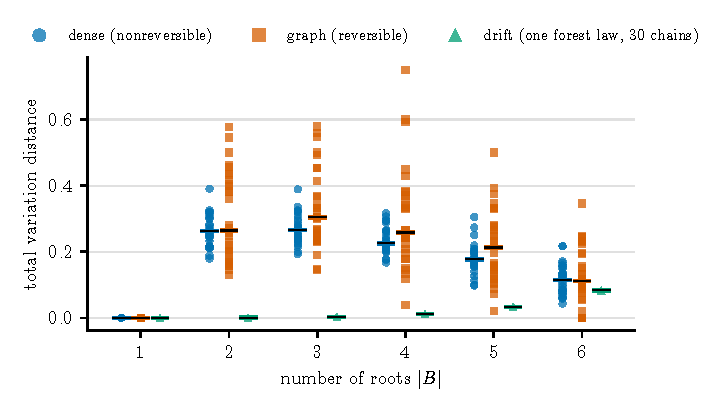
\includegraphics[width=0.85\textwidth]{figs/bias_tv.pdf}
\caption{Total variation distance between the stopped-walk forest law
\eqref{eq:closed} with seed $1$ and the weight-proportional law, for the
three families of \cref{tab:families} and root sets
$B=\{1\},\{1,2\},\dots,\{1,\dots,6\}$. Each point is one chain, and
the horizontal bars mark the medians; the drift family is shown once,
since its $30$ chains share one forest law. For $|B|=1$, the distance is
zero by \cref{thm:ab}.}
\label{fig:bias}
\end{figure}

For one root, the two laws agree, as \cref{thm:ab} requires.
With two roots, the median total variation distance is about $0.26$
for both the dense and graph families. With three roots, the medians
are about $0.27$ and $0.30$, respectively. The largest distance is
$0.75$, attained by one graph chain with four roots. Beyond three
roots, the median distances decrease to about $0.11$ at $|B|=6$.
These examples show that a stopped walk can differ substantially
from the target forest law even when the underlying chain is
reversible, as in the graph family.

The drift example has smaller distances for the chosen roots and
seed, increasing from $0.001$ at $|B|=2$ to $0.083$ at $|B|=6$.
This behavior depends on the contiguous roots and seed $1$; the next
experiment examines that dependence. All reported magnitudes concern
these chain families and root choices.

\subsection{Sensitivity}\label{sec:sens}
We vary the placement of the roots, the strength of the drift and the
connectivity of the graph; the script
\nolinkurl{robustness.py} reproduces the values below.

\emph{Placement.} For the same $30$ dense and $30$ graph chains, we
replace the nested roots and the seed $1$ by a uniformly random root set
of each size and a uniformly random seed in it. The median distances for
$|B|=2,\dots,6$ are $0.24$, $0.29$, $0.21$, $0.20$ and $0.13$ for the
dense family and $0.23$, $0.28$, $0.30$, $0.27$ and $0.16$ for the graph
family, close to those of \cref{fig:bias}, since these families do not
distinguish the labels of the states.

\emph{Drift.} The cycle does
distinguish them. \Cref{tab:drift} gives the range of the distance over
the seeds in the root set, for contiguous roots $\{1,\dots,b\}$ and for
roots spread evenly around the cycle, and for three drift strengths.
The small distances of \cref{fig:bias} occur only for the contiguous
roots and one seed; with another seed, or with spread roots, the
distance is of the same order as for the other families.

\emph{Connectivity.} For $30$ random connected graphs with edge
probability $0.30$, $0.45$ and $0.70$, the median distance for two roots
is $0.40$, $0.23$ and $0.23$, and the fraction of chains with lost mass
is $0.57$, $0.23$ and $0.13$; sparser graphs give larger distances and
more lost mass.

\begin{table}[!htbp]
\caption{Range of the total variation distance over the seeds in the
root set, for the drift cycle with forward weight $a$ and backward
weight $1$.}\label{tab:drift}
\centering
\footnotesize
\begin{tabular}{@{}llccccc@{}}
\toprule
$a$ & roots & $|B|=2$ & $3$ & $4$ & $5$ & $6$\\
\midrule
$1.5$ & contiguous & $0.03$--$0.23$ & $0.07$--$0.36$ & $0.13$--$0.44$ & $0.16$--$0.45$ & $0.01$--$0.37$\\
 & spread & $0.46$ & $0.56$ & $0.48$--$0.51$ & $0.26$--$0.39$ & $0.01$--$0.37$\\
\addlinespace[2pt]
$3$ & contiguous & $0.00$--$0.22$ & $0.00$--$0.29$ & $0.01$--$0.31$ & $0.03$--$0.30$ & $0.08$--$0.25$\\
 & spread & $0.30$--$0.31$ & $0.43$--$0.44$ & $0.40$--$0.47$ & $0.24$--$0.40$ & $0.08$--$0.25$\\
\addlinespace[2pt]
$6$ & contiguous & $0.00$--$0.14$ & $0.00$--$0.16$ & $0.00$--$0.17$ & $0.01$--$0.16$ & $0.02$--$0.14$\\
 & spread & $0.16$ & $0.27$--$0.28$ & $0.26$--$0.34$ & $0.14$--$0.26$ & $0.02$--$0.14$\\
\bottomrule
\end{tabular}
\end{table}

\subsection{Lost mass, effective sample size and an estimator}
Total variation distance alone does not identify whether correction
is possible. We therefore report two diagnostics in \cref{tab:lost}:
the unreachable target mass $q_W(S_1^c)$ and the limiting normalized
effective sample size of the inverse-completion weights. The former
measures the part of the target law that no reweighting can recover.
The latter measures weight dispersion on the reachable forests.
For $m$ independent draws $F^{(i)}\sim q_A$ with
weights $a_i:=1/\varphi_1(F^{(i)})$, the normalized effective sample size
$(\sum_ia_i)^2/(m\sum_ia_i^2)$ converges almost surely to
\[
\mathrm{ESS}/m:=\frac{(\E_{q_A}a)^2}{\E_{q_A}a^2}
=\Big(\sum_{F_0\in S_1}\frac{\bar q_W(F_0)^2}{q_A(F_0)}\Big)^{-1},
\qquad \bar q_W:=q_W(\cdot\mid S_1),
\]
which is the value reported in the table. Its interpretation concerns
weight dispersion: the precision of a particular estimate also
depends on the function $h$ and its association with the weights.

Lost mass is zero for all dense and drift chains. In the graph
family, it is positive for about half the chains with two or three
roots and reaches $0.75$. For the graph chain with four roots that
attains the largest total variation distance in \cref{fig:bias}, the
distance is entirely lost mass. Reweighting cannot reduce that
distance. On the reachable forests, the median limiting normalized
ESS is between $0.59$ and $0.95$ for the dense and graph families,
with a minimum of $0.31$.

\begin{table}[!htbp]
\caption{Lost target mass $q_W(S_1^c)$ for the graph family and
limiting normalized effective sample size $\mathrm{ESS}/m$ for the three
families, over the $30$ chains of each family. The lost mass is zero
for every dense and drift chain.}\label{tab:lost}
\centering
\footnotesize
\begin{tabular}{@{}ccccccccc@{}}
\toprule
& \multicolumn{3}{c}{graph: lost mass} & \multicolumn{5}{c}{$\mathrm{ESS}/m$}\\
\cmidrule(lr){2-4}\cmidrule(l){5-9}
$|B|$ & fraction $>0$ & median & max & dense med. & dense min & graph med. & graph min & drift\\
\midrule
$2$ & $0.53$ & $0.15$ & $0.58$ & $0.59$ & $0.31$ & $0.83$ & $0.69$ & $1.00$\\
$3$ & $0.57$ & $0.10$ & $0.58$ & $0.68$ & $0.43$ & $0.73$ & $0.52$ & $1.00$\\
$4$ & $0.37$ & $0$ & $0.75$ & $0.79$ & $0.59$ & $0.76$ & $0.34$ & $1.00$\\
$5$ & $0.20$ & $0$ & $0.50$ & $0.86$ & $0.72$ & $0.87$ & $0.47$ & $0.99$\\
$6$ & $0.03$ & $0$ & $0.20$ & $0.94$ & $0.83$ & $0.95$ & $0.62$ & $0.97$\\
\bottomrule
\end{tabular}
\end{table}

To illustrate the effect on an estimate, consider the expected size
of the seed's tree, $h(F_0):=1+|D_1|$, with $B=\{1,2\}$.
The first dense chain has complete support. Its target expectation
is $3.237$, while the uncorrected stopped-walk expectation is $4.359$.
The self-normalized correction converges to $3.237$. Across
$4{,}000$ replications with $m=200$ independent draws each, the
corrected estimate has mean $3.241$ and standard deviation $0.175$;
the limiting normalized ESS is $0.68$.

For the graph chain with the largest lost mass, $0.577$, the target
expectation is $1.923$ and the uncorrected expectation is $3.733$.
The correction converges to the conditional target $3.182$. Thus
correct weighting on the sampled forests does not resolve the loss
of the other forests. These calculations are generated by
\nolinkurl{estimator_demo.py}, which reuses the chains from
\nolinkurl{make_experiments.py} and uses random seed $1$ for the
replications.

\subsection{Checks}
We check the formulas first by enumeration. For every chain, root
set, and seed, the computed stopped-walk probabilities sum to one
and agree with the tree-law marginal obtained by enumerating the
arborescences. The largest discrepancy is $4.8\times10^{-15}$.
These checks verify the algebraic evaluations against a separate
enumeration of completed trees.

We also run \cref{alg:stopped} $200{,}000$ times on the first dense
chain with $|B|=2$ and seed $1$. This simulation uses only the forward
transition matrix. Of the $4{,}802$ expected counts, $755$ are below
$5$ and $79$ below $1$; the smallest is $0.26$. We therefore calibrate
the goodness-of-fit statistics with $2{,}000$ multinomial samples of
the same size from $q_A$, rather than a chi-squared approximation.
The reported upper-tail $p$-values have Monte Carlo standard errors
at most $0.011$.

The Pearson statistic is $4{,}818.1$, with simulated $p$-value $0.41$.
The maximum standardized deviation across forests is $3.52$, with
upper-tail $p$-value $0.995$. This maximum lies near the lower
$0.5\%$ tail of the simulated reference distribution and is unusually
small under $q_A$. The upper-tail test does not reject, but the small
maximum should not be read as evidence of better agreement. The
enumeration and the forward-walk simulation provide different checks;
the simulation statistics do not replace the deterministic checks.

\bibliographystyle{siamplain}
\bibliography{refs}
\end{document}
